\documentclass[12pt,a4paper,class,twoside,openany]{report}
\usepackage[utf8]{inputenc}
\usepackage{amsmath}
\usepackage{amsfonts}
\usepackage{amssymb}
\usepackage{graphicx}
\author{Eventati Team}
\title{Eventati Project Documentation}
\begin{document}
\pagenumbering{roman}
\begin{abstract}
\paragraph*{\hspace{.9 cm} }
 "Eventati"  is a Social Event Directory not only a website but also a mobile application to manage and deal with events via internet, provides with most of social functionalities by 25Jan revolutionists to all eventatians.Because of  problems that face most of people when they miss some of his important events in all life fields .So "Eventati"  aimed to collect all events in one site, get localization of each event through map, and to allow communications between all friends.
 "Eventati" also allows users to invite their friends and follows others and also provides the ability to create their own events, invite their friends to attend events, share events among their friends what make the events spread widely. "Eventati" automates a lot of repeating tasks and collecting the data together in one place where you can access any time.
 \paragraph*{\hspace{.9 cm} } Mobile Application describes a feasible way of integrating mobile networks with the Internet, in order to deal with events  that  allow mobile devices to receive common web transactions and allows Internet peers to be notified of mobile generated events. Mobile application of "Eventati"  facilitates  accessing for mobile users to access the events through their devices, while Mobile applications are hugely popular for customer service. We thought in mobile application as a result of the great revolution in mobile application development and we have finished developing our application. "Eventati" web Team has finished developing user management system and event management system.
\paragraph*{\hspace{.9 cm} } "Eventati" consists of three major teams. Every team uses open Source technologies. Firstly, Web Team uses three major tools, Django framework, Pinax with Django and python as a programming language. Secondly, Mobile Team uses Appcelerator Titanium with Java Script to create a version of the application for each targeted   device. Finally, Design team uses advanced Graphic editing tool (Photoshop).
In the future we will add some functions to our project such as Mozilla Firefox add-ons, aversion for tablets, procedures like how to reach to specific Event, enabling transportation and on-line payment for events to allow users to pay to get event's tickets.
\end{abstract}
\cleardoublepage
\chapter*{Acknowledgements}
\paragraph*{\hspace{.9 cm} }
In the name of Allah the Most Gracious, the Most Merciful.We would like to express our eternal appreciations towards our beloved parents and family who have always been there for us, for all unconditional encouragement and patience. Thank you for being ever so understanding and supportive.\\
We must give our high, respectful gratitude to our supervisor "Dr. Haitham El-Ghareeb" for the valuable guidance and advice. He inspired us greatly to work in this project. His willingness to motivate us contributed tremendously to our project. We also would like to thank him for showing us some example that related to the topic of our project.\\
\paragraph*{\hspace{.9 cm} }We owe a great many thanks to many people who helped us and supported us during "Eventati" Project.
Firstly,Endless thanks especially from the design team to Eng. Shaimaa Adel for the guidance and help throughout the project. We have learned a lot form her and she gave us precious advices in order to improve ourselves and become better designers.
Secondly,The Mobile team and Web team tends thanking to Eng.Elsayed Gamal for his valuable time and effort and for supporting the whole group to work using open source technologies.
Thirdly,Great thanks to Harvest and ILC company for being one of the sponsors to the project by providing labs and convenient place.
\tableofcontents
\cleardoublepage
\listoffigures
\cleardoublepage
\listoftables
\cleardoublepage
\pagenumbering{arabic}
\cleardoublepage
\chapter{Introduction}
\section{Need for the Project}
 \paragraph*{\hspace{.9 cm} } Today  and after the noted  increasing in  events  in different fields of life  ,it became difficult to us to handle  these  events  manually and if  we try  that  we will miss some of  those events ,so  thought about tool that handles our events and brings it where we are. This project tends to social Network for its important. Statistically By March 10-2011, there were more than 24 million FaceBook users in the Arab World [Arab Advisor Groups] , Figure \ref{fg:1-1} presented in page \pageref{fg:1-1} shows Statistic of Social Network in USA,Jordan and Egypt. Social Network Sites like  FaceBook, Twitter, Google+, LinkedIn , MySpace and REDDIT are in every where ,Figure \ref{fg:1-2} presented in page \pageref{fg:1-2} shows logos of most famous  social Networks[avtec].Today’s youth are spending a great deal of time using these sites to access virtual life and also after revolution of 25 Jan Social Network Sites are widely increasing and also from  our belief with  importance of communication with others. The problem statement we noticed is when anyone wants to announce about event there is no dedicated place that s/he can invite people through it, he simply makes to every event websites or Web-page and to avoid missing events that I want to attend, So that we need "Eventati".    
  
   \begin{figure}
	\begin{minipage}[b]{0.5\linewidth}
	\centering
	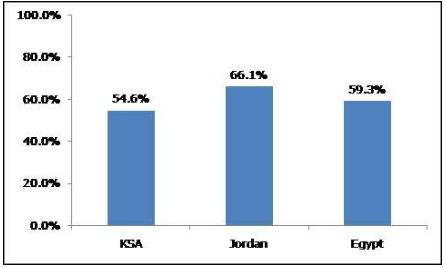
\includegraphics[scale=.6]{1-1}
	\caption{Statistic of Social Network in 2011}
	\label{fg:1-1}
	\end{minipage}
	\hspace{0.5cm}
	\begin{minipage}[b]{0.5\linewidth}
	\centering
	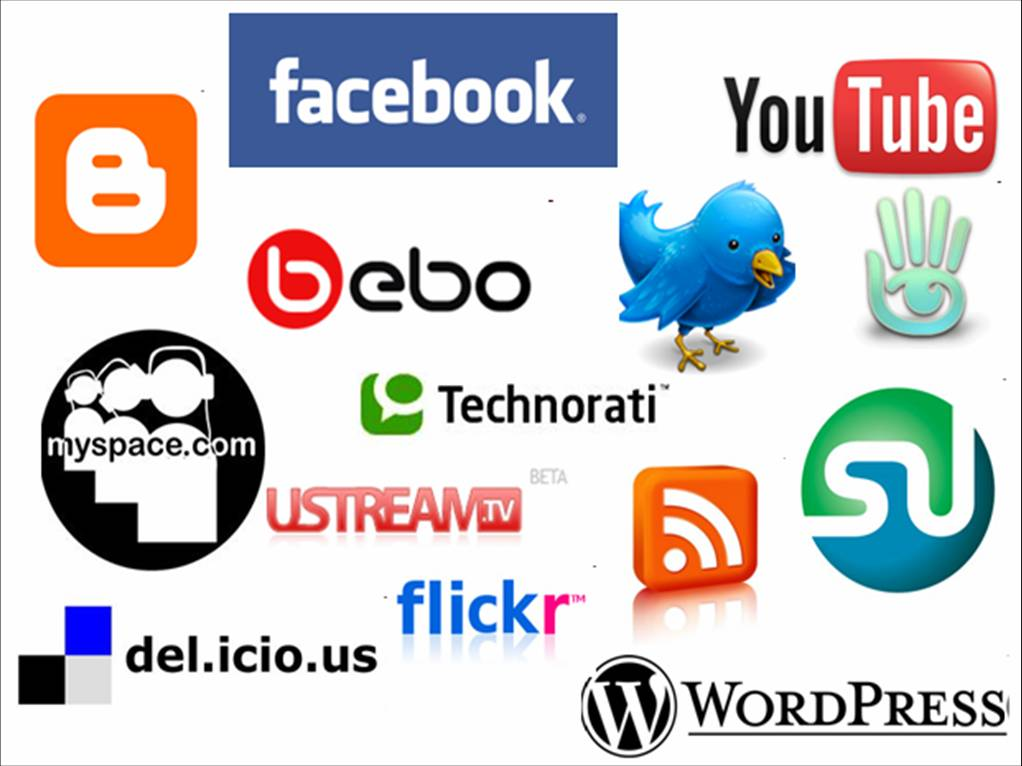
\includegraphics[width=\textwidth]{1-2.jpg}
	\caption{Social Networks}
	\label{fg:1-2}
	\end{minipage}
	\end{figure}
	
\section{Aim of the Project}
\paragraph*{\hspace{.9 cm} } After the revolution of internet technology we found that created web and mobile application especially social website become important component in the life of every one as we with this technology can follow events in any field we have interested in it. After creating this project everyone can use this project to create his event and share it with his friends easily  in efficient way and also become a follower for any event that takes place around you."Eventati" makes life easier to you, so it can enable you following your interested events where and when ever they are held.

\section{Integration between Mobile and Web}
\paragraph*{\hspace{.9 cm} } To complete the purpose of our project (bringing events where we are),thinking in integration between our web application  and mobile application as it easier for anyone to take mobile device with him/her in any place than taking personal computer and  the using of mobile application very simple for any user,So integration is important. Mobile application must connect to web services (Data Base) which in the web application. By using standard protocols like SOAP protocol by reading WSDL by XML. Message.response representations from the according web service protocols (WSDL, SOAP, and UDDI) have to be translated into corresponding requests response data types of the agent system, and vice versa.To integrate between web and mobile application by using XML RPC.
 XML RPC: It's a set of implementations that allow software running on disparate operating systems, running in different environments to make procedure calls over the Internet.
It's remote procedure calling using HTTP as the transport and XML as the encoding. XML-RPC is designed to be as simple as possible, while allowing complex data structures to be transmitted, processed and returned.


\section{Thesis Structure}
\paragraph*{\hspace{.9 cm} }In This Chapter we presented the need, aim and the integration between Web and Mobile Application. Next Chapters go as follow:
\\
\textbf{Chapter Two:} Methodology has been presented Agile Methodologies, Scrum, meetings, Stories and Testing.
\\
\textbf{Chapter Three:} Technologies have been presented open Sources in Web and Mobile components.
\\
\textbf{Chapter Four:} Web Components have been presented introduction, user requirements, websites back end design, interface Design, implementation and testing.
\\
\textbf{Chapter Five:} Mobile components have been presented introduction, user requirement, user interaction with mobile App and  Simple code.
\\
\textbf{Chapter Six:} Design components have been presented introduction, logo design, mobile icons and site layout.
\\
\textbf{Chapter Seven:} Integration between web and Mobile presents introduction, integration methods,  XML RPC and code samples.
\\
\textbf{Chapter Eight:} project outcomes present the output of "Eventati" representing as screen Shots of outcomes of this project.
\\
\textbf{Chapter Nine:} presents Conclusion and Future Works that we will do in the future In chaa Allah.
\cleardoublepage
\chapter{Methodologies}
\section{Agile Methodologies}
\paragraph*{\hspace{.9 cm} }Every project must follow dedicated method to make a great project. Traditionally, Waterfall  used as a methodology to develop a project, but waterfall has some limitations to be used until now, so agile methods will be used in almost project. In the Agile Method, communication between customers and the members of the project team is very vital and essential. Agile management in the project helps you defining the project easily and clearly with stakeholders and team members. The basic designs are kept simple and clean and feedback starts immediately as does software testing. This enables the project to be implemented early as changes are made immediately to any part of the project that requires it. The Agile method also allows the product to be launched after each stage and allows parallel analysis. In Contrast the waterfall that has no stopping and if end-testing doesn't go well, you better think about starting all over again. One of the leading agile software development processes is Scrum.Figure \ref{fg:2-1} presented in page \pageref{fg:2-1} shows different between Waterfall and Scrum [flicker].
\begin{figure}[htbp]
\begin{center}
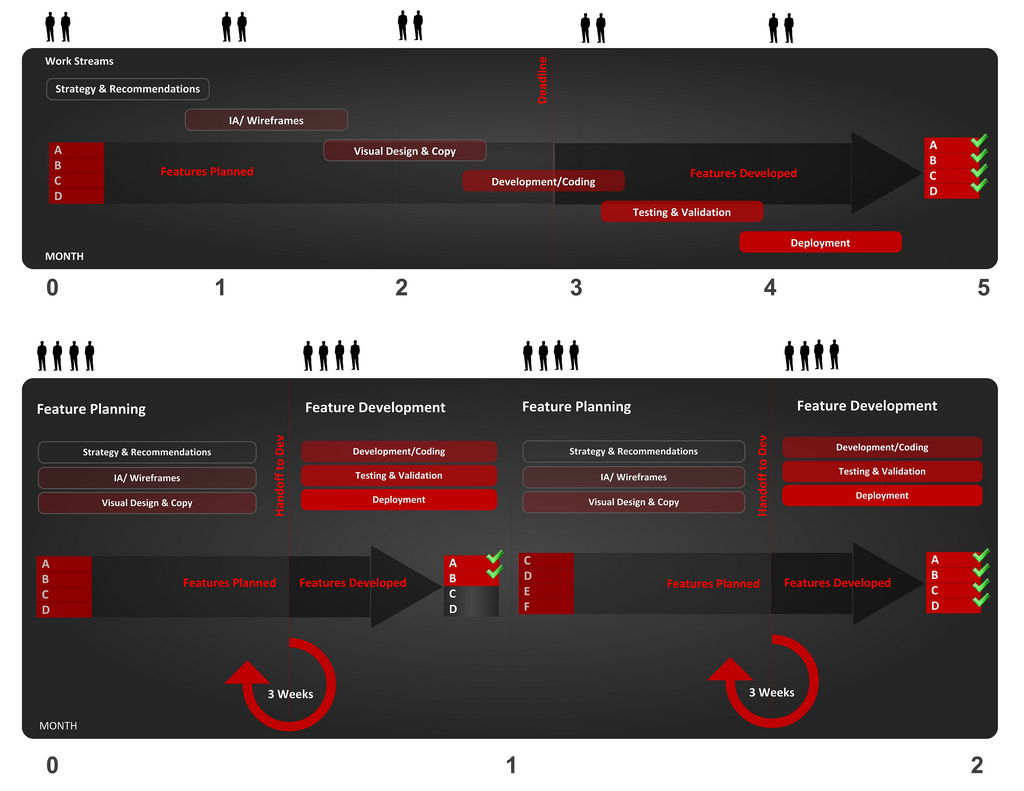
\includegraphics[scale=2,angle=90,width=\textwidth]{2-1}
\caption{Waterfall and Scrum }
\label{fg:2-1}
\end{center}
\end{figure}

\section{SCRUM}
 \paragraph*{\hspace{.9 cm} } Scrum has become recognized as one of the best project management frameworks for handling rapidly changing or evolving projects. Especially useful on projects with lots of technology or requirements. It is a method for mapping software projects and product or application development. It has one of the best agile development practices using today. In any project we can get features request from customers, executives or even other team members. In Scrum features are written from the perspective of the end user, therefore features are known as user stories, in collection of all these user stories are called product backlog. Product backlog is wish list of all things would make the product great. Once we have a product backlog or a wish list, we must determine which specific user stories we want to achieve first which has a priority.  
To build this product we need to have one or more people and has rules need to be followed:
\begin{enumerate}
\item Product owner - helps making  sure the right features that represent user's requirements.
\item Scrum Master - to make sure the project is progressing smoothly and facilities release planning.
\item Developer - to build the project.
\item Tester - tested to make sure works rights
\item Customer - use it and helpfully to pay for it.
\end{enumerate}
\paragraph*{\hspace{.9 cm} } Scrum works with product Backlog which is nothing more than a list of features the weak high user's stories, then break down product backlog into one or more release backlogs and for agave release you further release backlogs into numbers of sprint backlogs and then your manner progressively sprint use Burn down Charts and have daily scrum meetings to ensure everything in on track after each sprint. We have a sprint retrospective to find everything [Hamid Shojaee]. Figure \ref{fg:2-2} presented in page \pageref{fg:2-2} shows all the processes in SCRUM. To Apply Scrum on "Eventati" ,the Figure \ref{fg:2-3} presented in page \pageref{fg:2-3} shows one of our scrum team members and Figure \ref{fg:2-4} presented in page \pageref{fg:2-4} shows Product Backlog of "Eventati".
\begin{figure}
\begin{center}
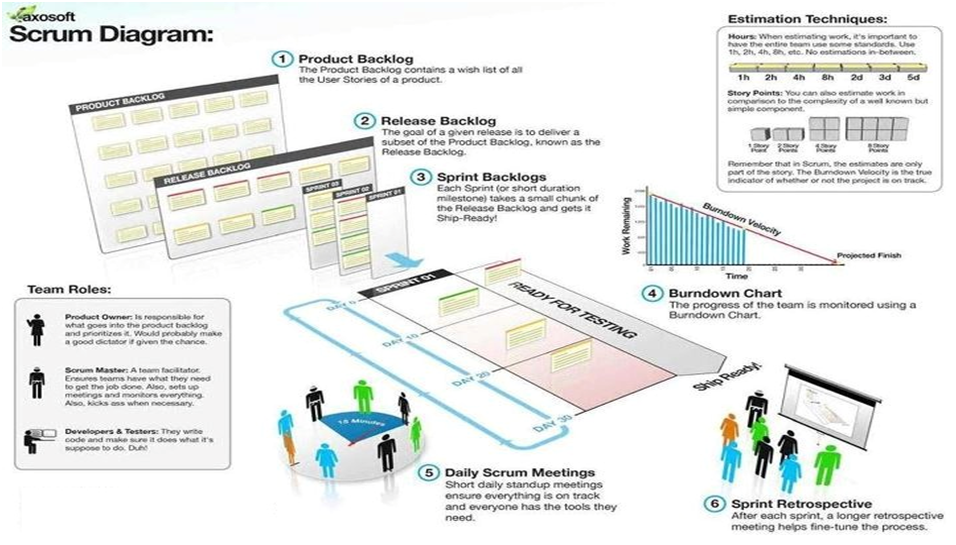
\includegraphics[angle=90,width=4.5 in]{2-2}
\caption{SCRUM Diagram}
\label{fg:2-2}
\end{center}
\end{figure}\\
 \begin{figure}
	\begin{minipage}[b]{0.5\linewidth}
	\centering
	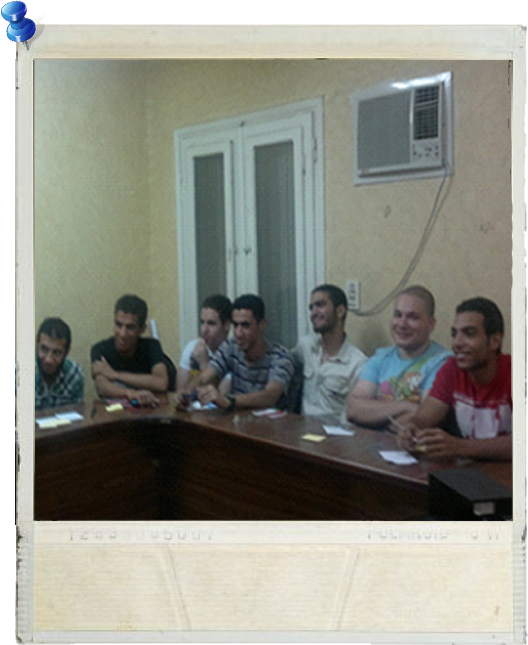
\includegraphics[height=3.5 in]{2-3}
	\caption{Scrum Team Members}
	\label{fg:2-3}
	\end{minipage}
	\hspace{0.5cm}
	\begin{minipage}[b]{0.5\linewidth}
	\centering
	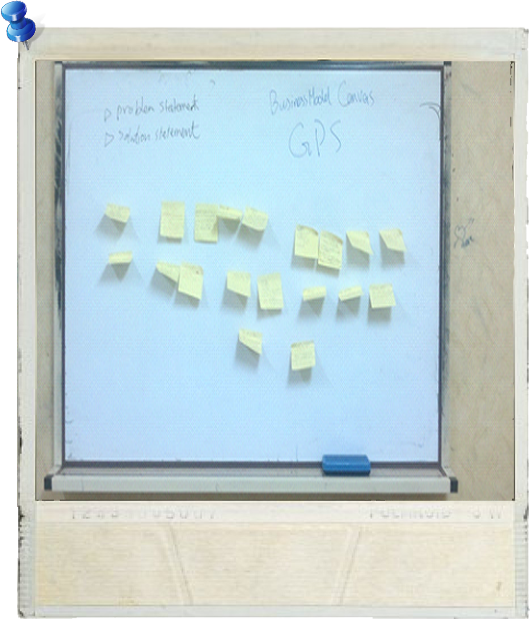
\includegraphics[height=3.5 in]{2-4}
	\caption{Product Backlog  Of "Eventati" }
	\label{fg:2-4}
	\end{minipage}
	\end{figure}
 \\
\subsection{Meetings}
 \paragraph*{\hspace{.9 cm} } According to scrum we made a lot of meetings almost 20 meetings all team meet together to complete and work for "Eventati" Project.
We began used Xmind tool beginning with Meeting5 and we had more than 15 meetings by the supervisor  "Dr Haitham A.E-Ghareeb" and other meetings with team members only.
Every meeting has been recorded with date,place,Start and end time , attendances,last tasks that we discussed and had to do this and new tasks that we will make them.
For first five  meetings didn't make it with Xmind tool,then we reminded them shortly .
\begin{enumerate}
\item Meeting 1: we talked about project and what it's dimension then we revised java Script and discussed communication tool with others.
\item Meeting 2: we explained  Scrum and divided the team into three major teams Web,Design and Mobile team   and discussed MVC and language tool Web2by that the web team used it firstly.
\item Meeting 3: we talked about SVN , Google code, discussed the different types of Remote Execution Methods and standards: XML-RPC, SOAP (implements WSDL), Restful (implements WSDL), JSON,then Design team presented first work Mockups on paper that it showed System web site and all team impressed with their work they will update it with Cacoo tool next time .
\item Meeting 4: "Dr Haitham" meets with each team individually and discussed about tools and what each team will study and be suitable for the "Eventati" project .
\item Meeting 5: Place: ILC,date: 2-10-2010 at 10.45 pm We discussed that day Features of the project and determined weekly meeting for each team.
\item Meeting 6: Figure \ref{fg:2-5} presented in page \pageref{fg:2-5} showed that discussion of three things. Firstly, we discussed analysis that we need Use case, Activity and sequence Diagrams. Secondly, we discussed the Test driven development (TDD) how to test, why should we first test, why should another one test, why test first is good. Thirdly, we discussed some issues that we have met, one of these is if an event is cancelled, it must be in updating not make deleting operation.
\item Meeting 7:Figure \ref{fg:2-6} presented in page \pageref{fg:2-6} showed that according to Mobile Team we discussed about titanium that we used it to build "Eventati" mobile application and distributed tasks on team, Web team decided using Django instead of using web2by because it was easy and fast in development and performance otherwise web2by was not customized and need URL function Mobile and discussed  these tasks Install the environment, subversive, Events Manager to be finished and user Registration using layout.
\item Meeting 8:Figure \ref{fg:2-7} presented in page \pageref{fg:2-7} showed that it
determined Events entities,source Code management,Product Backlog version 1  and  suing "yamel" tool for design team.
\item Meeting 9:Figure \ref{fg:2-8} presented in page \pageref{fg:2-8} showed that we discussed Logo rules and new technologies that we used like pianx and bootstrap then  mobile team needed icons and discussed about presentation and Documentation.
\end{enumerate}
\textbf{These teams with out "DR.Haitham" the supervisor:}
\begin{enumerate}
\item Meeting 1:Figure \ref{fg:2-9} presented in page \pageref{fg:2-9} showed that the first team with out our supervisor "Dr Haitham" that we rearranged new tasks and distributed them on all team members. UML,Attributes,Icons and determined tasks to next meeting we needed a Survey  ,Class,Sequence,Activity Diagram and complete home page (Web and Design Team).
\item Meeting 2:Figure \ref{fg:2-10} presented in page \pageref{fg:2-10} showed the initial diagrams Activity , sequence and class Diagrams and we needed to revise it with "Dr Haitham".
\item Meeting 4:Figure \ref{fg:2-11} presented in page \pageref{fg:2-11} showed that we discussed Main ,Home pages,Logan and Slogan .we had notes to be discussed with "Dr Haitham".
\item Meeting 5:Figure \ref{fg:2-12} presented in page \pageref{fg:2-12} showed that we 
discussed Video Or slide Show to represent our system site to users ,then we discussed Slogan of "Eventati" that every member in team  suggested at least two slogan and at the end we voted the slogan "Every Moments Something Happens" that took the highest votes.
\end{enumerate}
The Last Two Meeting be collected every things that we done with out "Dr Haitham" to Show them to him.
\begin{enumerate}
\item Meeting 10:Figure \ref{fg:2-13} presented in page \pageref{fg:2-13} showed that this meeting was with "DR Haitham" discussed  presentation according to with design team about fonts and position of slogan and logo and rearranged of slides.According to mobile team that they needed a vital pictures not Screen shoots and need a spacial Use Case and Diagrams.According to web team that we needed statistical for presentation,MVC Just one Slide,Benefits of RSVP need to updated.
\item Meeting 11:Figure \ref{fg:2-14} presented in page \pageref{fg:2-14} showed that this also was with "DR Haitham" there was final updating to this presentation of "Eventai",Use Case Diagrams  and talked about how to represent it.
\\ \textbf{Great Thanks To "DR Haitham" for helping us too much and not saving his efforts at all.}
\end{enumerate}
\begin{figure}
\begin{center}
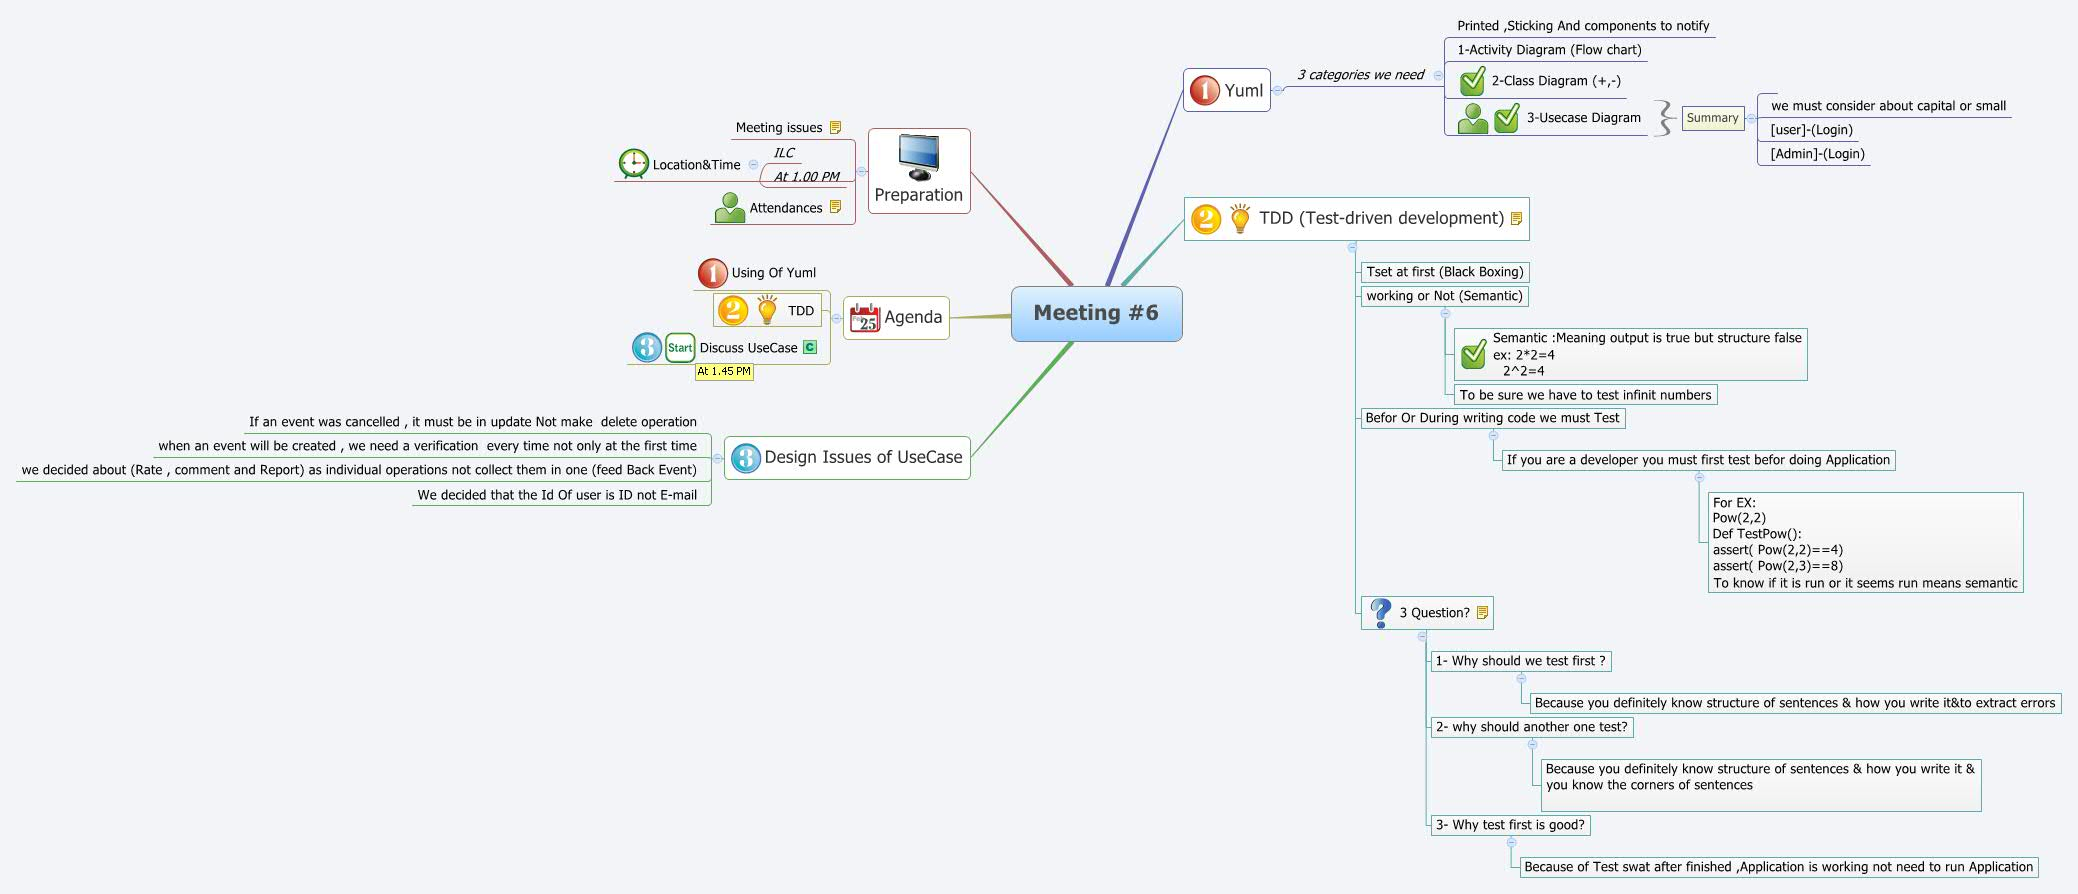
\includegraphics[angle=90, width=3.5 in]{2-5}
\caption{Meeting 6}
\label{fg:2-5}
\end{center}
\end{figure}
 \begin{figure}
\begin{center}
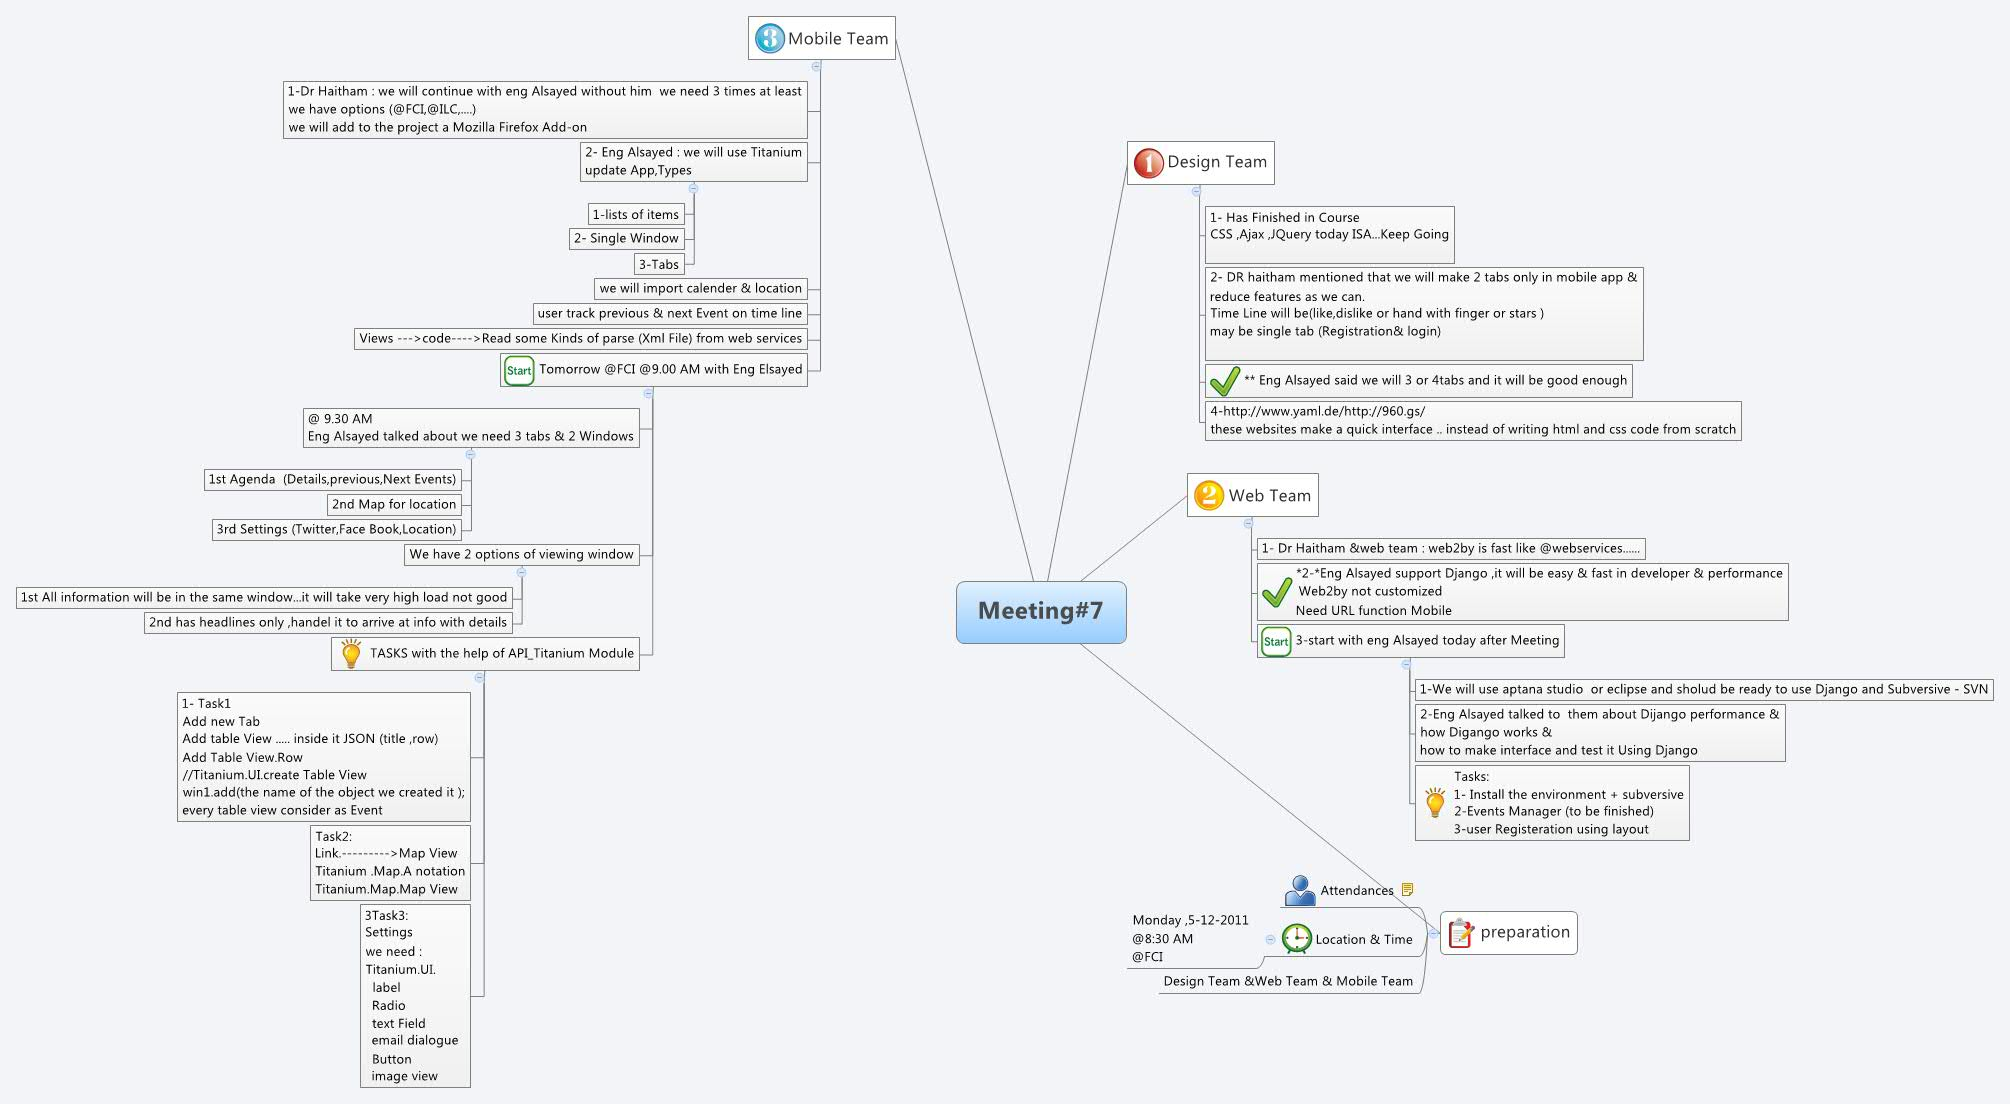
\includegraphics[angle=90, width=4 in]{2-6}
\caption{Meeting 7}
\label{fg:2-6}
\end{center}
\end{figure}
\begin{figure}
\begin{center}
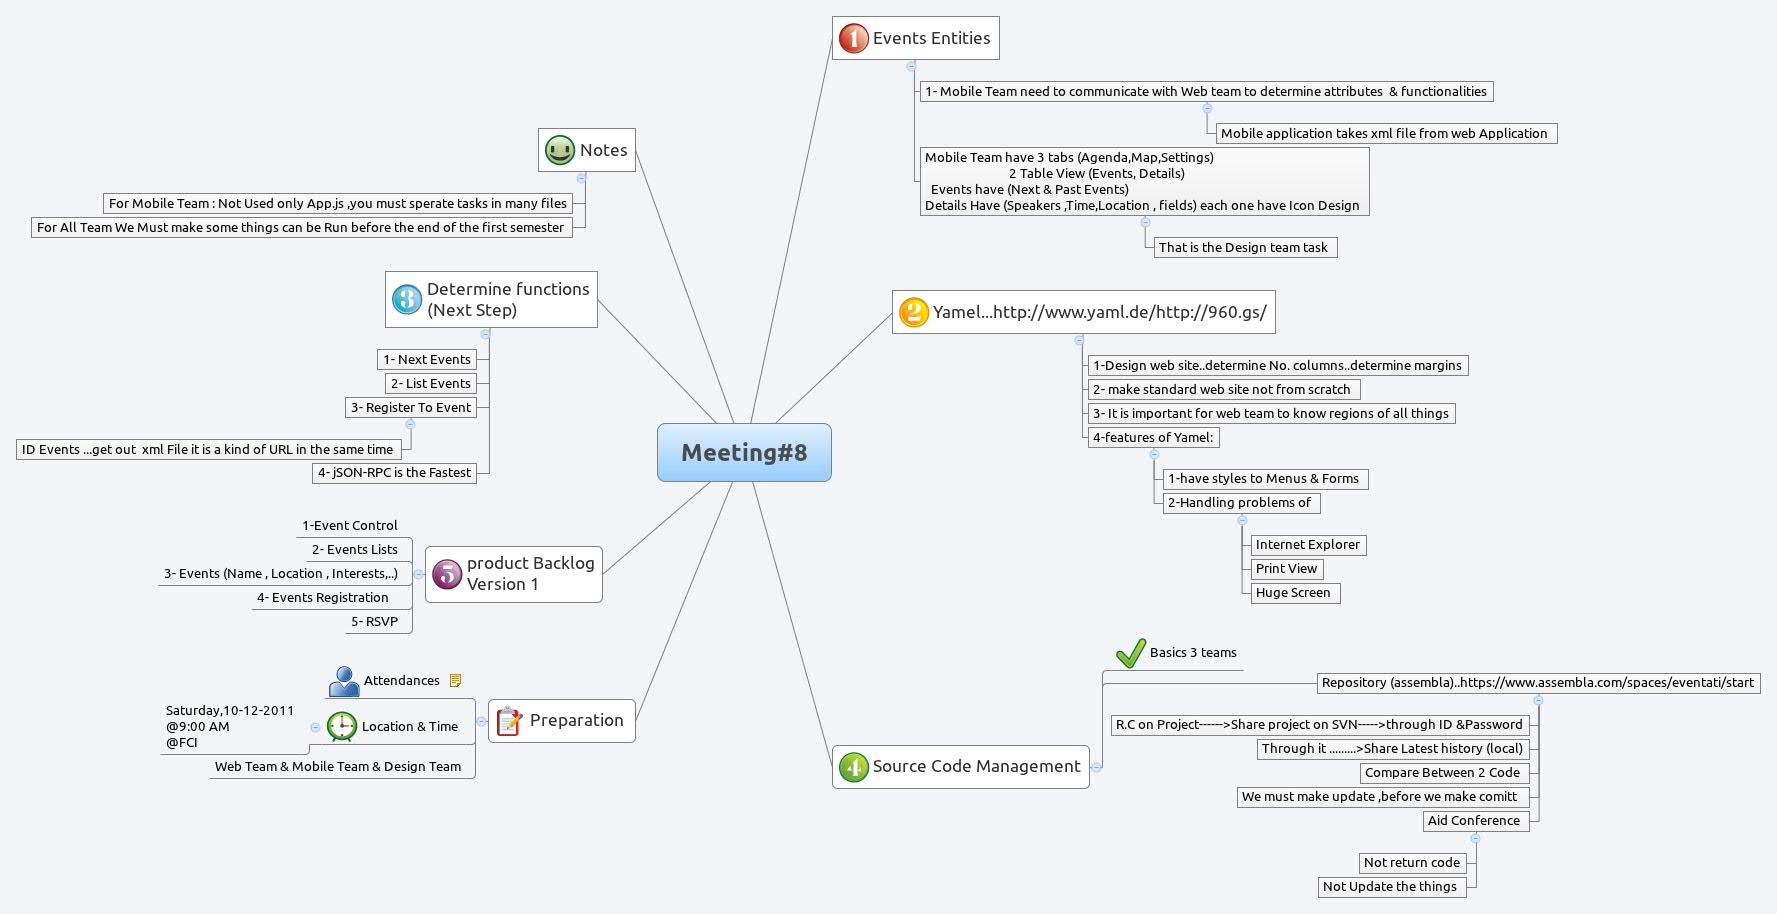
\includegraphics[angle=90, width=4 in]{2-7}
\caption{Meeting 8}
\label{fg:2-7}
\end{center}
\end{figure}
\begin{figure}
\begin{center}
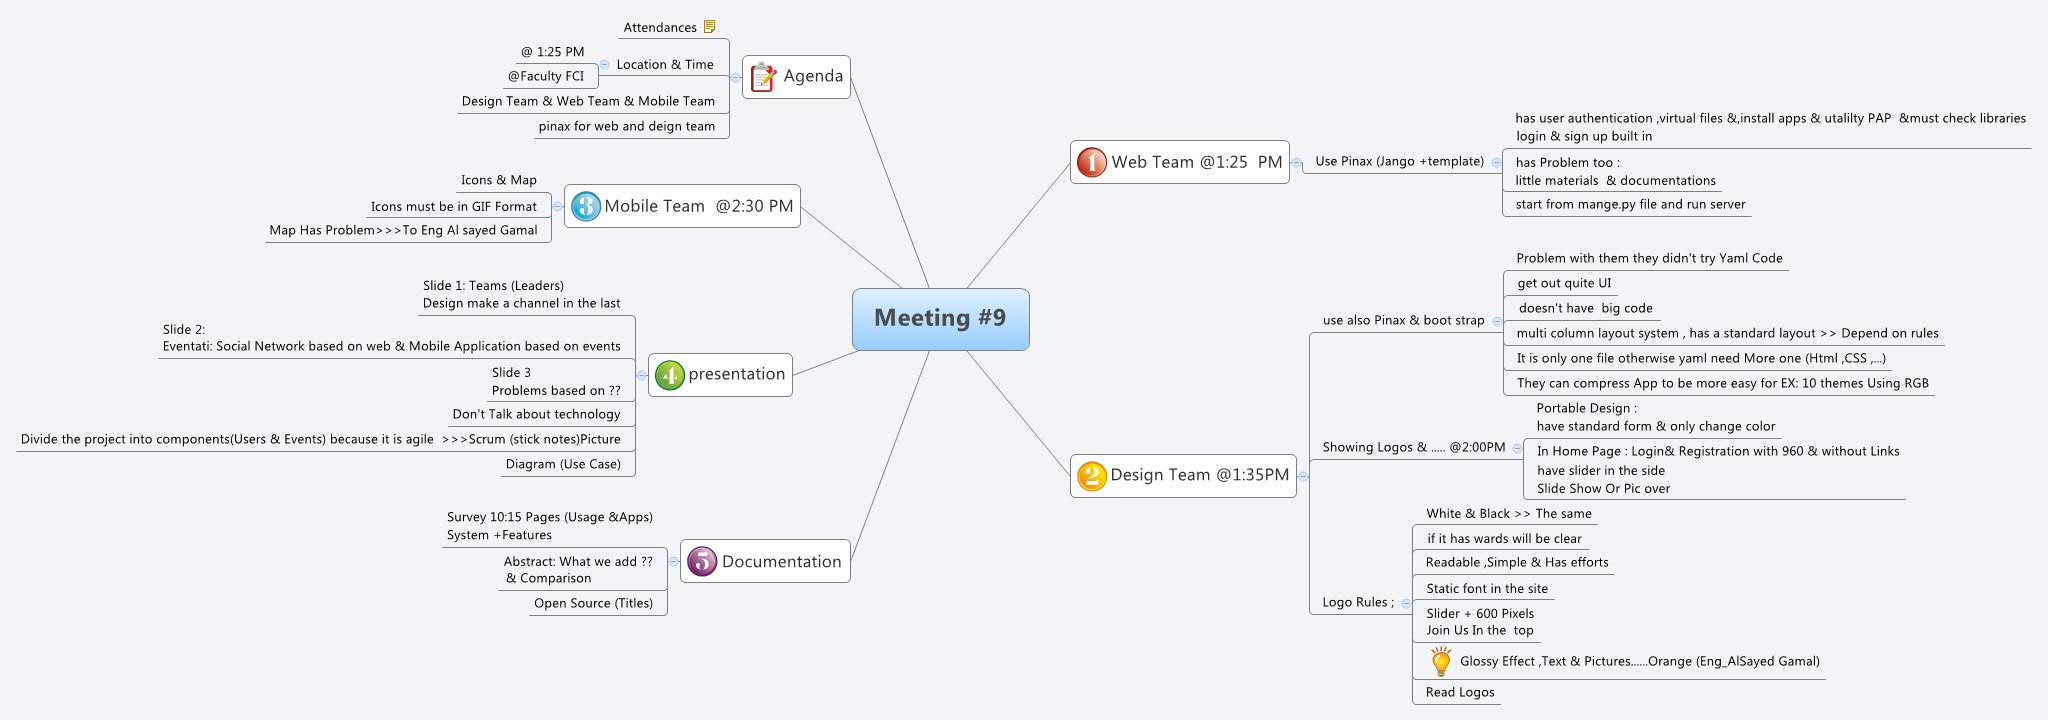
\includegraphics[angle=90, width=5 in,height=8 in]{2-8}
\caption{Meeting 9}
\label{fg:2-8}
\end{center}
\end{figure}
\begin{figure}
\begin{center}
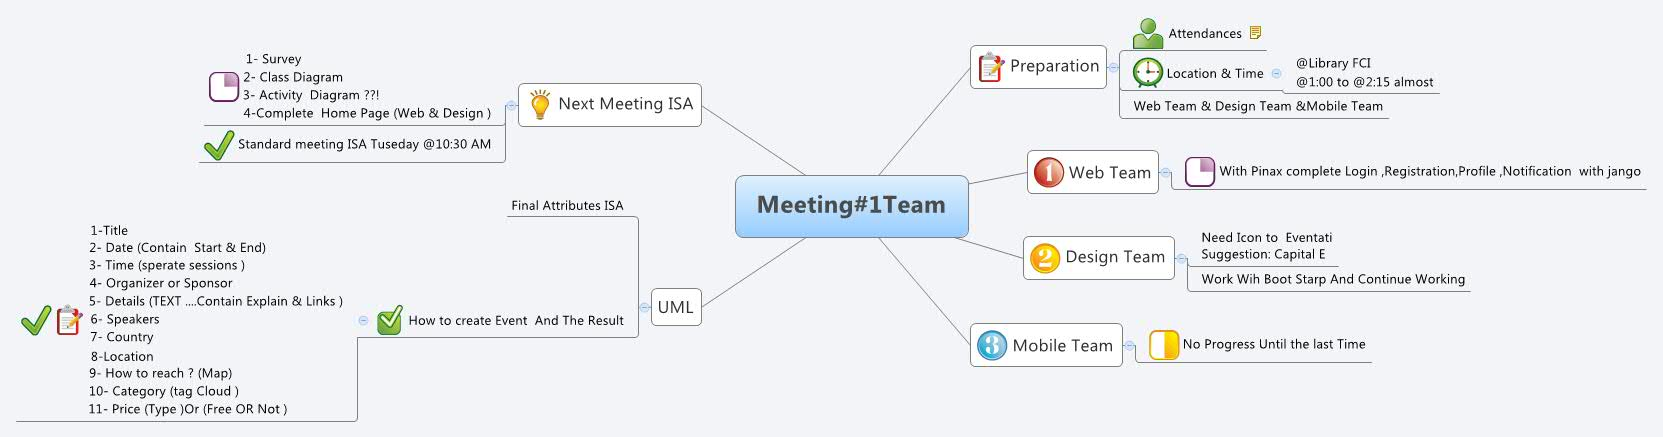
\includegraphics[angle=90, width=2.40 in,height=8 in]{2-9}
\caption{Meeting 1 Only Team}
\label{fg:2-9}
\end{center}
\end{figure}
\begin{figure}
\begin{center}
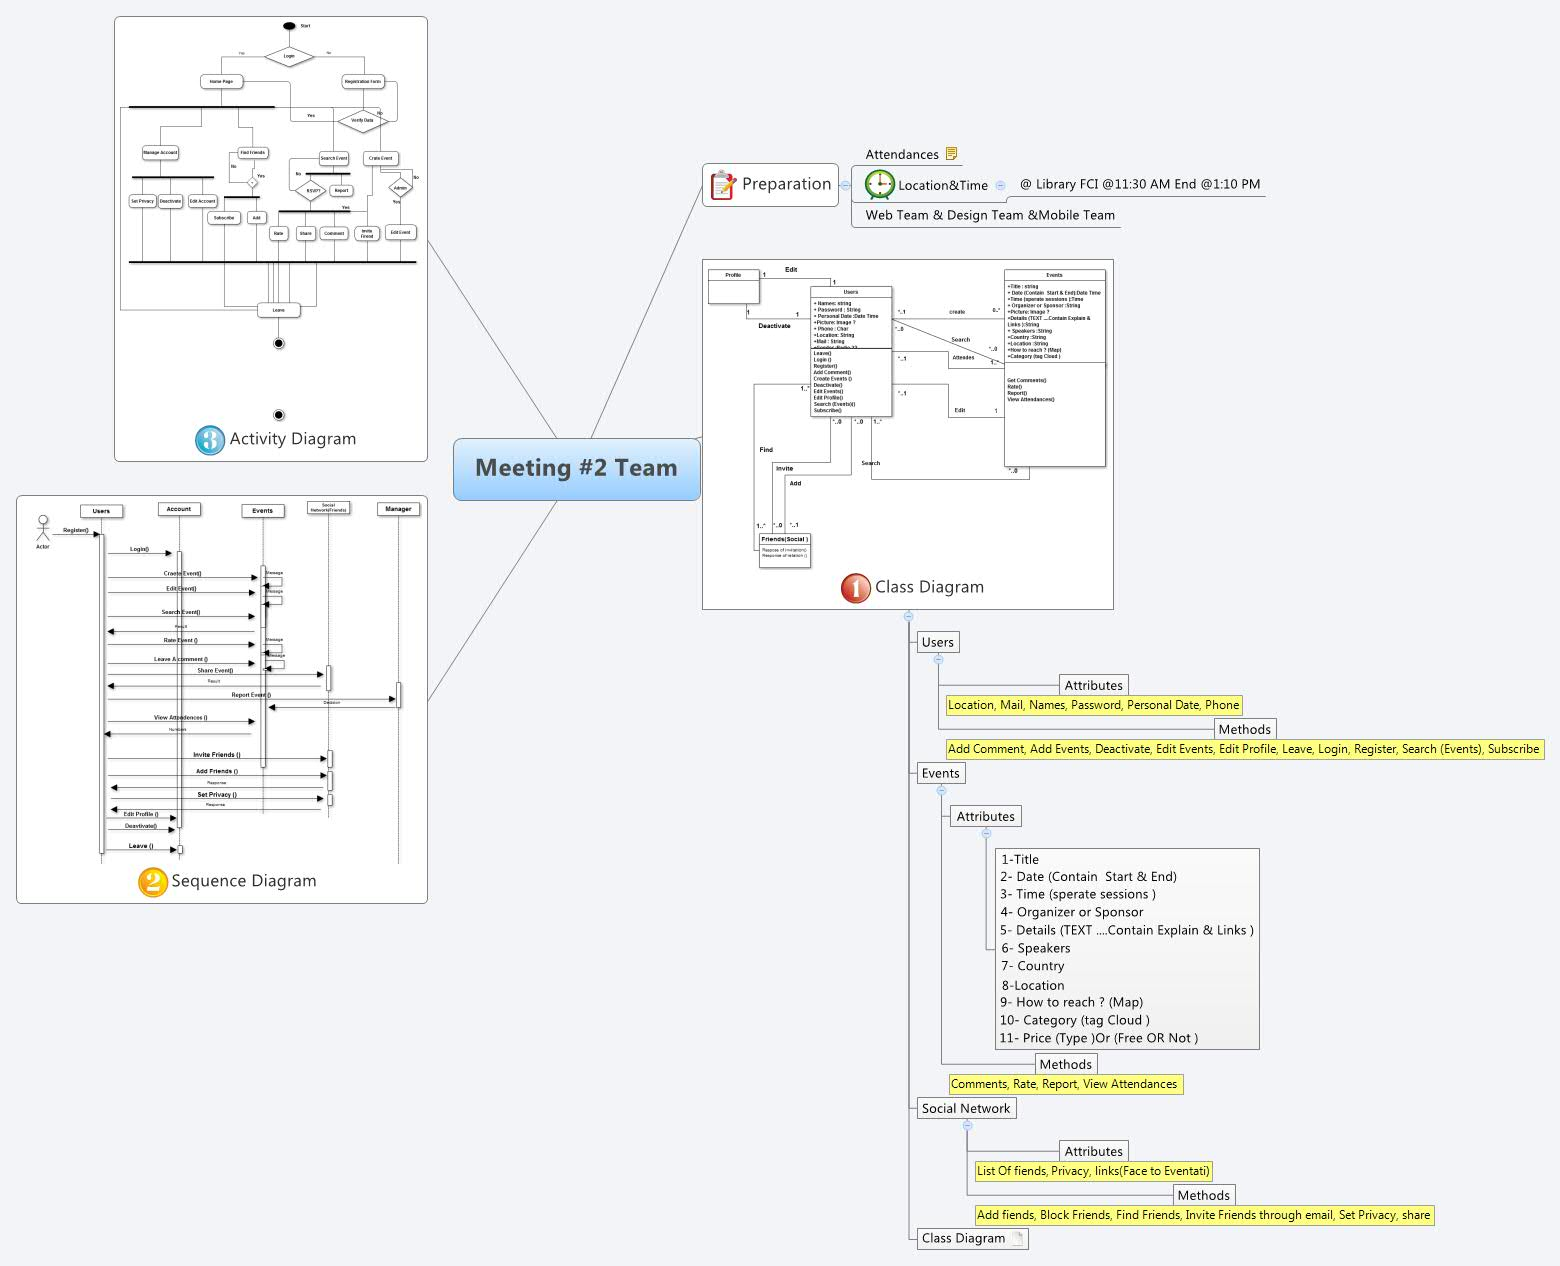
\includegraphics[angle=90, width=5 in]{2-10}
\caption{Meeting 2 only Team}
\label{fg:2-10}
\end{center}
\end{figure}
\begin{figure}
\begin{center}
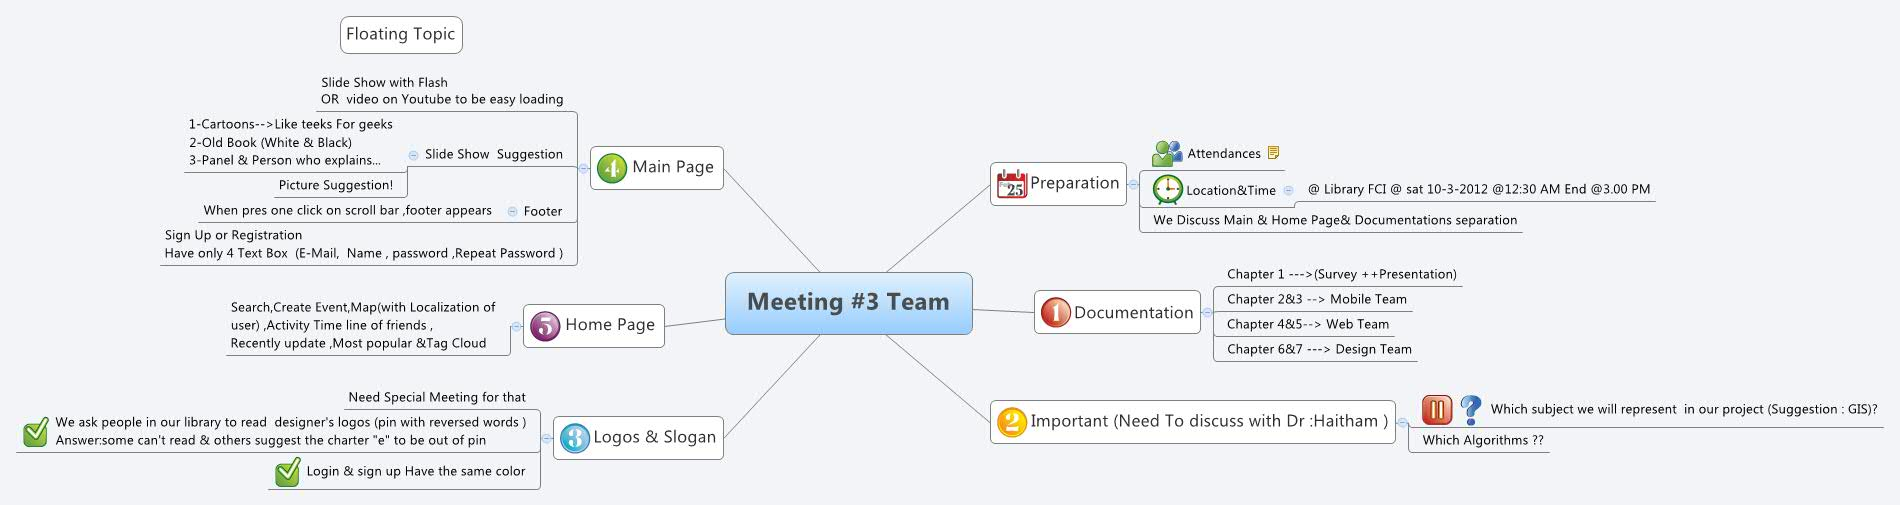
\includegraphics[angle=90, width=2.25 in ]{2-11}
\caption{Meeting 3 only Team}
\label{fg:2-11}
\end{center}
\end{figure}
\begin{figure}
\begin{center}
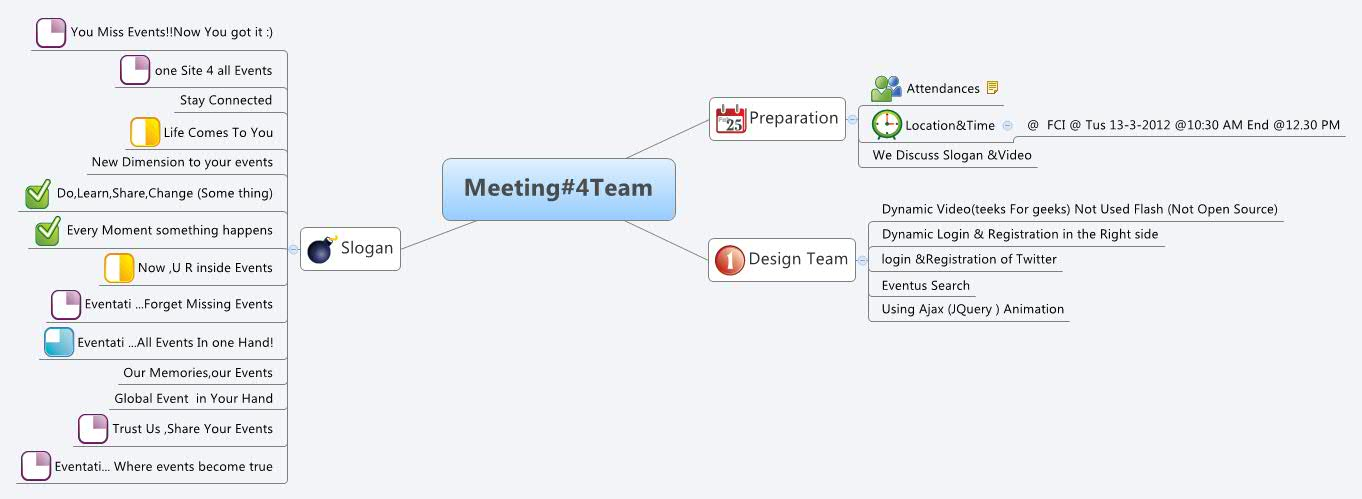
\includegraphics[angle=90, width=2.80 in ]{2-12}
\caption{Meeting 4 only Team}
\label{fg:2-12}
\end{center}
\end{figure}
\begin{figure}
\begin{center}
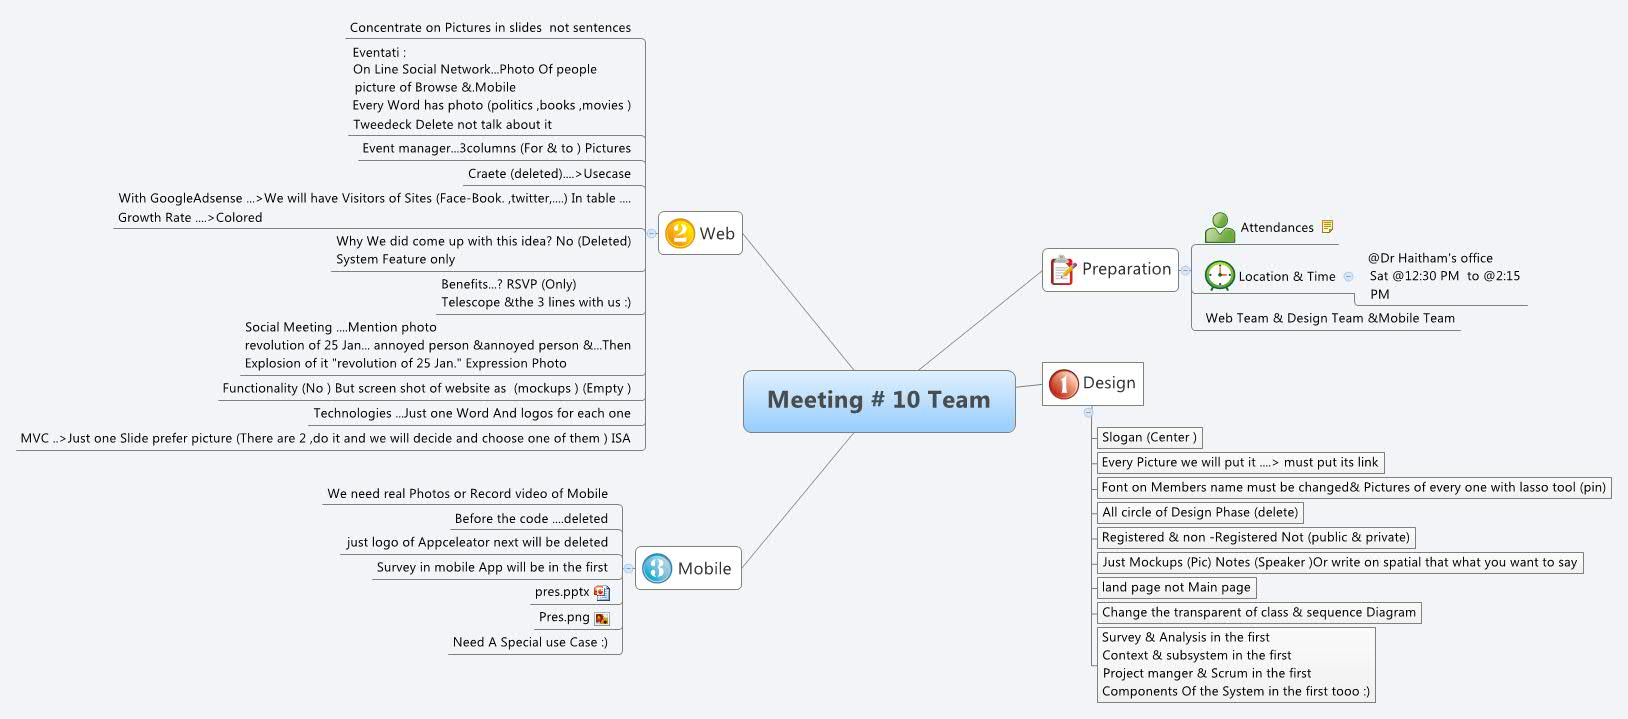
\includegraphics[angle=90, width=4 in]{2-13}
\caption{Meeting 10}
\label{fg:2-13}
\end{center}
\end{figure}
\begin{figure}
\begin{center}
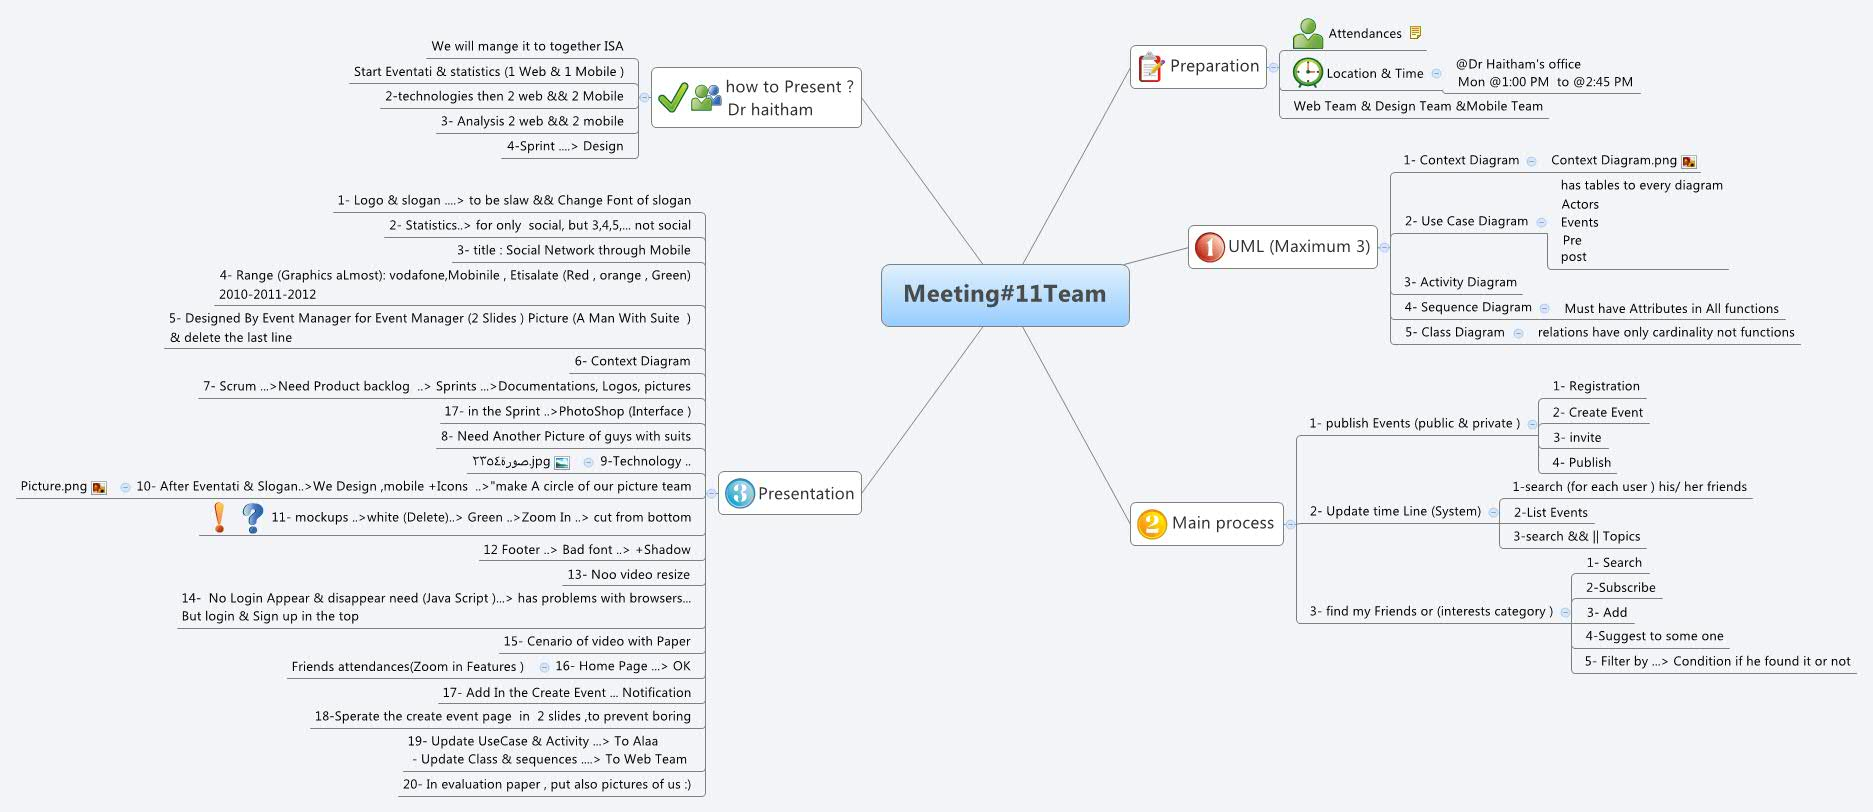
\includegraphics[angle=90, width=3.75 in]{2-14}
\caption{Meeting 11}
\label{fg:2-14}
\end{center}
\end{figure}

\textbf{\subsection{Stories:}}
\paragraph*{\hspace{.9 cm} }Stockholders write user stories; user stories mean features of our project.
 User Stories of "Eventati":
 \begin{itemize}
\item[•] User can create Events.
\item[•] User can invite friends.
\item[•] User can publish Events through Mail, Social network or "Eventati".
\item[•] User can get location of each event and friend.
\item[•] User can follow new friends.
\item[•] Use can rate each event.
\item[•] User can leave a comment in each event.
\item[•] User can confirm attending with RSVP.
\item[•] System can notify all subscribes.
\item[•] System can recommend places, friends, events to Authorized users
 \end{itemize}
\textbf{ \subsection{Testing:}}
  \paragraph*{\hspace{.9 cm} } When our software is completing , it must be tested against the system requirements to see if it fits the original goals. As well as this kind of conformance testing, it's a good idea to see if our software can be broken via its external interfaces , this helps to protect us against accidental or malicious abuse of the system when it's been deployed.
\\
  \paragraph*{\hspace{.9 cm} } Testing is intended to show that a program does what it is intended do and to discover program defects before it is put into use. We need testing to validate, defect Verify and validate our project. Other important rules we need to differentiate between inspections and testing. Software Inspection is Static Verification while Software Testing is dynamic Verification. There are many different types of testing. The prominent ones this series will cover are unit tests and integration tests.
\\

 \paragraph*{\hspace{.9 cm} } Another point of decision is deciding whether to do test-first or test-after. Test-first is where you write the necessary tests to demonstrate proper behaviour of the code BEFORE you write the code to solve the problem at hand. Test-after is when you've already written the code to solve the problem, then you go back and create tests to make sure the behaviour of the code you wrote is correct.
\cleardoublepage 
\chapter{Technologies}
\section{Web Technology}
 In web application we used major open source technologies python, Django framework, and pinax  you can  take some information about them in  following lines.
 \subsection{Python}
 
\begin{figure}
	\begin{minipage}[b]{0.5\linewidth}
	\centering
	
\includegraphics[scale=.9]{3-1}
	\caption{Python Logo}
	\label{fg:3-1}
	\end{minipage}
	\hspace{0.5cm}
	\begin{minipage}[b]{0.5\linewidth}
	\centering
	
\includegraphics[width=\textwidth]{3-2}
	\caption{Django Logo}
	\label{fg:3-2}
	\end{minipage}
	\end{figure}
 \paragraph*{\hspace{.9 cm} }Python is an interpreter, object-oriented and high-level programming language with dynamic semantics. Its high-level built in data structures, combined with dynamic typing and dynamic binding; make it very attractive for Rapid Application Development, as well as for use as a scripting or glue language to connect existing components together. Python's simple, easy to learn syntax emphasizes readability and therefore reduces the cost of program maintenance. Python supports modules and packages, which encourages program modularity and code reuse. The Python interpreter and the extensive standard library are available in source or binary form without charge for all major platforms, and can be freely distributed.
 Often, programmers fall in love with Python because of the increased productivity it provides. Since there is no compilation step, the edit-test-debug cycle is incredibly fast. Debugging Python programs is easy: a bug or bad input will never cause a segmentation fault. Instead, when the interpreter discovers an error, it raises an exception. When the program doesn't catch the exception, the interpreter prints a stack trace. A source level debugger allows inspection of local and global variables, evaluation of arbitrary expressions, setting breakpoints, stepping through the code a line at a time, and so on. The debugger is written in Python itself, testifying to Python's introspective power. On the other hand, often the quickest way to debug a program is to add a few print statements to the source: the fast edit-test-debug cycle makes this simple approach very effective [Python].
\subsection{Django} 
 \paragraph*{\hspace{.9 cm} } Because of Django was developed in a fast-paced newsroom environment, it was designed to make common Web development tasks fast and easy .Django is an open source web application framework, written in Python, which follows the model-view-controller architectural pattern. It was originally developed to manage several news-oriented sites for The World Company of special place in USA, and was released publicly under a BSD license in July 2005; the framework was named after guitarist Django Reinhardt. In June 2008 it was announced that a newly formed Django Software Foundation will maintain Django in the future.
Django's primary goal is to ease the creation of complex, database-driven websites. Django emphasizes reusability and "pluggability" of components, rapid development, and the principle of don't repeat yourself. Python is used throughout, even for settings, files, and data models. Django also provides an optional administrative create, read, update and delete interface that is generated dynamically through introspection and configured via admin models[Adrian Holovaty and  Jacob Kaplan-Moss].
 Django Application:
\\ Django is a free web framework written in python has its own typical structure
\begin{enumerate}
\item You have an application folder "apps", where all your application are.
\item In the static folder you have all static files like, css, js, images etc..
\item In custom folder we put our own logic with we overwrite some specific application.
\item In template folder we put our templates, how the website should look like.
\item The files in the root project tree, like settings and urls.py are global for the project.
\end{enumerate}
This is a common structure, but you can make it however you want, this is not a requirement. In Django you can overwrite most of the behaviour [Django Application]and[ by book keeper]. 
\begin{figure}
\begin{center}
\fbox{
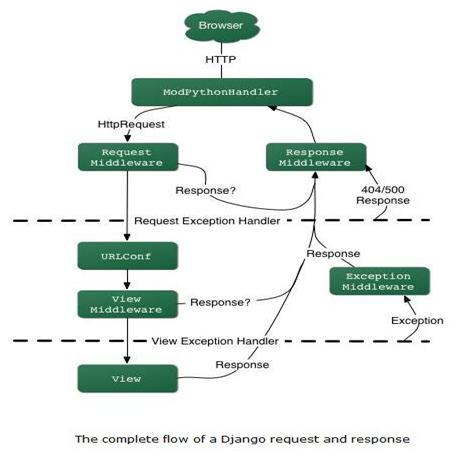
\includegraphics[height=4.5 in]{3-3}
}
\caption{Django Request and Response}
\label{fg:3-3}
\end{center}
\end{figure}
\begin{figure}
\begin{center}
\fbox{
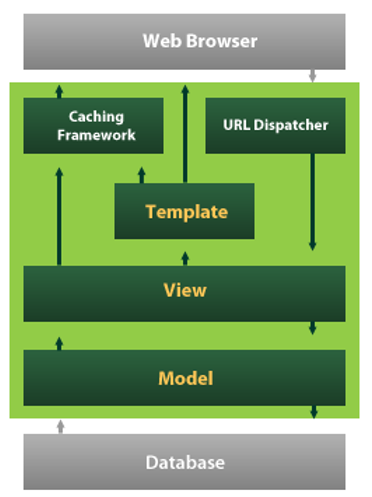
\includegraphics[height=2.5 in]{3-13}
}
\caption{Django Application}
\label{fg:3-13}
\end{center}
\end{figure}

\begin{figure}
\begin{center}
\fbox{
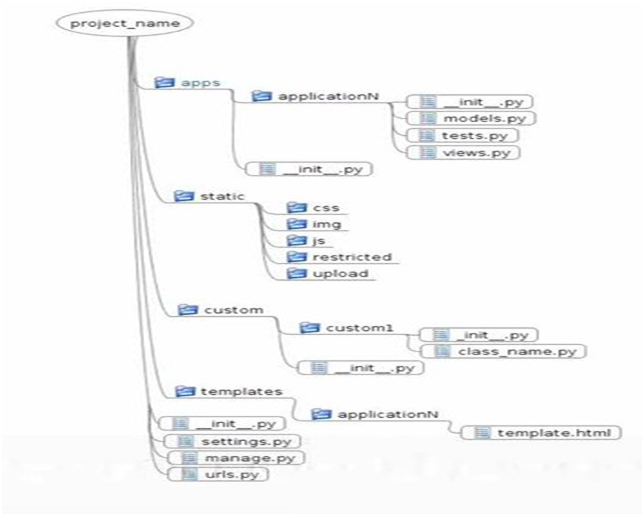
\includegraphics[height=3 in]{3-14}
}
\caption{Django Application Structure}
\label{fg:3-14}
\end{center}
\end{figure}

\subsection{The MVC Design Pattern}
 \begin{figure}
\begin{center}
\fbox{
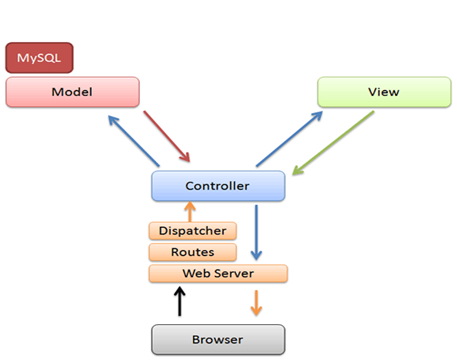
\includegraphics[height=3 in]{3-4}
}
\caption{ MVC Design Pattern}
\label{fg:3-4}
\end{center}
\end{figure}

\paragraph*{\hspace{.9 cm} } Let's dive in with a quick example that demonstrates MVC,The first thing to note is that we split it over three Python files
(models.py,views.py,urls.py) and an HTML template latest-books.html.models.py (the database tables), views.py (the business logic), urls.py (the URL configuration) and latest-books.html (the template).\\ \\ \\
 \begin{figure}
\begin{center}
\fbox{

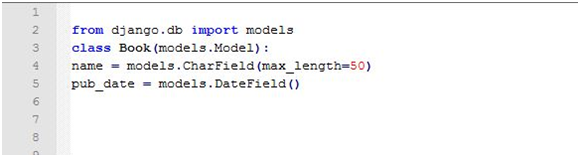
\includegraphics[height=1 in]{3-5}
}
\caption{models.py (the database tables)}
\label{fg:3-5}
\end{center}
\end{figure}
 
\begin{figure}
\begin{center}
\fbox{
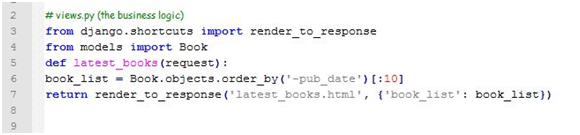
\includegraphics[height=1 in]{3-6}
}
\caption{views.py (the business logic)}
\label{fg:3-6}
\end{center}
\end{figure}

 \begin{figure}
\begin{center}
\fbox{
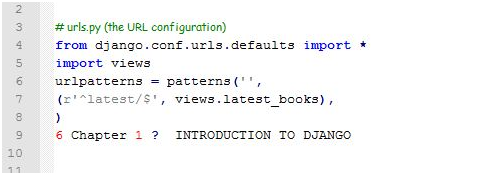
\includegraphics[height=1.5 in]{3-7}
}
\caption{urls.py (the URL configuration)}
\label{fg:3-7}
\end{center}
\end{figure}

\begin{figure}
\begin{center}
\fbox {
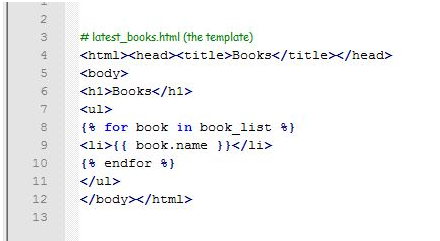
\includegraphics[height=2.5 in]{3-8}
}
\caption{latest-events.html (the template)}
\label{fg:3-8}
\end{center}
\end{figure}

\begin{itemize}
\item The models.py file contains a description of the database table, represented by a Python class. This class is called a model. Using it, you can create, retrieve, update, and delete records in your database using simple Python code rather than writing repetitive SQL statements.

 \item The views.py file contains the business logic for the page. The latest-books() function is called a view.
\item The urls.py file specifies which view is called for a given URL pattern. In this case, the
URL /latest/ will be handled by the latest-books() function. In other words, if your domain is example.com, any visit to the URL [http://example.com/latest/] will call the
latest-books() function.
\end{itemize}

\paragraph*{\hspace{.9 cm} } The latest-books.html file is an HTML template that describes the design of the page.
It uses a template language with basic logic statements for example, .
Taken together, these pieces loosely follow a pattern called Model-View-Controller (MVC).Simply put, MVC is way of developing software so that the code for defining and access in data (the model) is separate from request-routing logic (the controller), which in turn is separate from the user interface (the view).
 A key advantage of such an approach is that components are loosely coupled. Each distinct piece of a Django-powered Web application has a single key purpose and can be changed independently without affecting the other pieces. For example, a developer can change the URL for a given part of the application without affecting the underlying implementation. A designer can change a page's HTML without having to touch the Python code that renders it.A database administrator can rename a database table and specify the change in a single place rather than having to search and replace through a dozen files.
\subsection{Pinax}
\begin{figure}
\begin{center}
\fbox{

\includegraphics[height=1 in]{3-9}
}
\caption{pinax}
\label{fg:3-9}
\end{center}
\end{figure}
\paragraph*{\hspace{.9 cm} } A platform for rapidly developing websites Pinax is an open-source platform built on the Django Web Framework. By integrating numerous reusable Django application and providing starter projects and infrastructure tools, Pinax takes care of the things that many sites have in common so you can focus on what makes your site different. Pinax has been used for everything from social networks to conference websites, and from intranets to on-line games. Pinax provides:
\begin{itemize}
\item[•]	standard project layout for consistency and easy deployment
\item[•]	starter projects that can be used as the basis for any Django website as well as some tailored to community sites, company sites, intranets and sites in closed beta 
\item[•]	reusable applications providing both back-end functionality and user-facing components
\item[•]	default templates to enable quick prototyping
including applications for:
\begin{itemize}
\item	account management
\item	open id
\item	e-mail verification
\item	password management
\end{itemize}
\item[•]	profiles
\item[•]	notifications
\item[•]	activity streams
\item[•]	private betas / waiting lists
\item[•]	tagging
\item[•]	wikis
\end{itemize}
[James Tauber]
\newpage

 \section{Mobile Technology}
 \subsection{Appcelerator}
 \begin{figure}
	\begin{minipage}[b]{0.5\linewidth}
	\centering
	
\includegraphics[scale=.55]{3-10}
	\caption{Appcelerator Logo}
	\label{fg:3-10}
	\end{minipage}
	\hspace{0.5cm}
	\begin{minipage}[b]{0.5\linewidth}
	\centering
	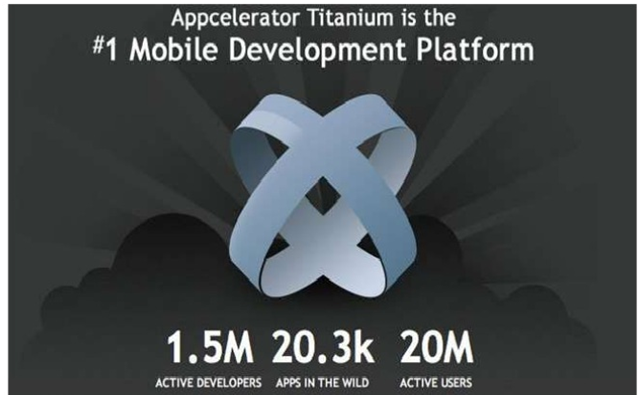
\includegraphics[width=\textwidth]{3-11}
	\caption{Titanium Logo}
	\label{fg:3-11}
	\end{minipage}
	\end{figure}
  \paragraph*{\hspace{.9 cm} } "Eventati"  Mobile team used open source technologies,because of open source is better quality, higher reliability, more flexibility and  lower cost. There are many problem that we faced and overcame with titanium,problems such as [Appcelerator,Inc]:             
  \begin{itemize}
\item[•] Building Cross Platform Mobile Solutions.
\item[•] Building Applications in cost-effective manner.
\item[•] Providing best of breed user Experience.
\item[•] Building a sustainable, maintainable for application and team .
 \\  \paragraph*{\hspace{.9 cm} }  Appcelerator is an open source developer platform designed to allow programmers to create native applications that function across a wide range of devices.Appcelerator Titanium Mobile is one of several phone web based application framework solutions allowing web developers to apply existing skills to create native applications for iPhone and Android. Yet, while using the familiar JavaScript syntax, developers will also have to learn the Titanium API[Richard Bateman].
 The language that "Eventati" mobile team  used
 Appcelerator==JS+TitaniumAPIs        
We used titanium with java script,write code in JSON. JSON (JavaScript Object Notation) is a lightweight data-interchange format. It is easy for humans to read and write. It is easy for machines to parse and generate. It is based on a subset of the JavaScript Programming Language. The code gets compiled using the device SDKs so the deployed application runs natively on the phone not only android but also IOS. 

\end{itemize}
 Today you need to be in three places at once: On-line, On-phone, and On-desktop
The html/css/javascript code that makes up the core application logic and UI, All of this can be done through Appcelerator Titanium [Viktor, ShoutEm CEO].

\begin{figure}
\begin{center}
\fbox{
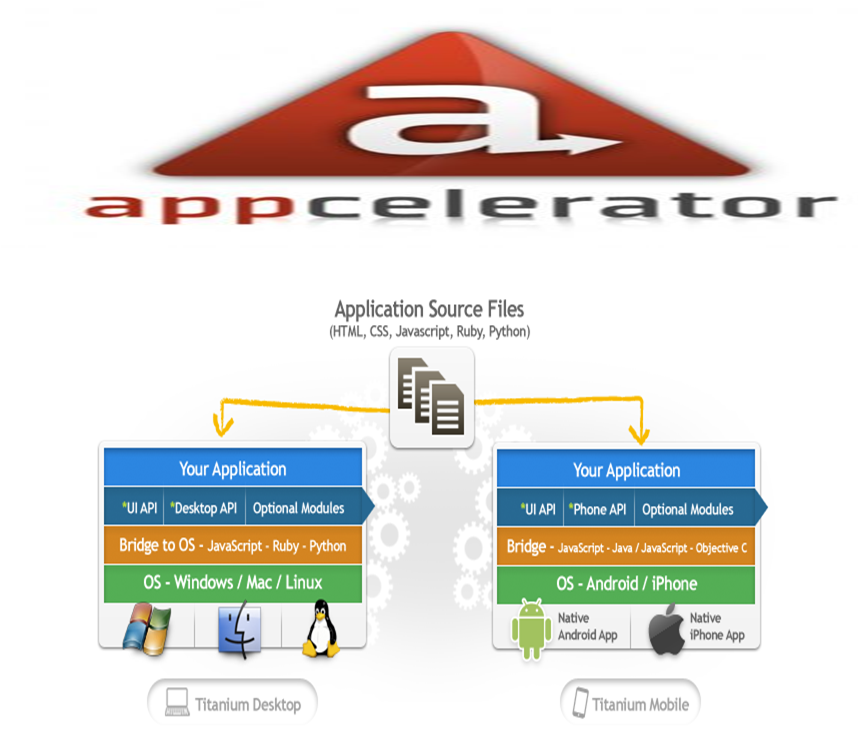
\includegraphics[height=3.5 in]{3-12}
}
\caption{Appcelrator of Application Sources File}
\label{fg:3-12}
\end{center}
\end{figure}
\cleardoublepage
\chapter{Web Components}
\section{Introduction}

\paragraph*{\hspace{.9 cm} }  An API, or “ Application Program Interface, is a set of routines and protocols that provide    building blocks for computer programmers and web developers to build software applications. In the past, APIs were largely associated with computer operating systems and desktop applications. In recent years though, we have seen the emergence of web API. Website development is an extensive term for the work involved in developing a web site for the World Wide Web. Web development services can range from developing a simple static web page of plain content to the most complex web-based internet applications, e-commerce businesses, or social network services.Moreover, for larger organizations and businesses, web development teams can consist of hundreds of web developers, whereas smaller organizations may only require a single web master and a secondary member assigned to related job positions such as a graphic design or a server testing. Web development is a collaborative effort between various departments rather than the domain of a single specific department.
\section{System Requirements}
 \subsection{Publish Event}
 \paragraph*{\hspace{.9 cm} }   Registration  on the web application  is the first functional requirement of our system after it come other requirement some of them are functional and another are Non-functional, we  will  make a trip in our system and  specify it's requirement (functional,Non-functional).
After registration the system gives to user an optional requirement it is completing user's profile it isn't barrier for the user to do other process of the system.
After that user should create his event and try to publish his event via many different ways such as share event via "Eventati" network or other social network and after this the event will be appear to the user friend in all network s/he shared his event on it and he will receive notification about his friend acceptance and joining his event all this process only for registered user.Figure \ref{fg:4-0} presented in page \pageref{fg:4-0} shows how to get System Requirements."Eventati" Consists of four components user management, Event management,Social Network and Mobile Application shown in Figure \ref{fg:4-1} presented in page \pageref{fg:4-1} shows Context Diagram. Figure \ref{fg:4-2} presented in page \pageref{fg:4-2} shows Web-UseCase-PublishEvent.
\begin{figure}
\begin{center}
\fbox{
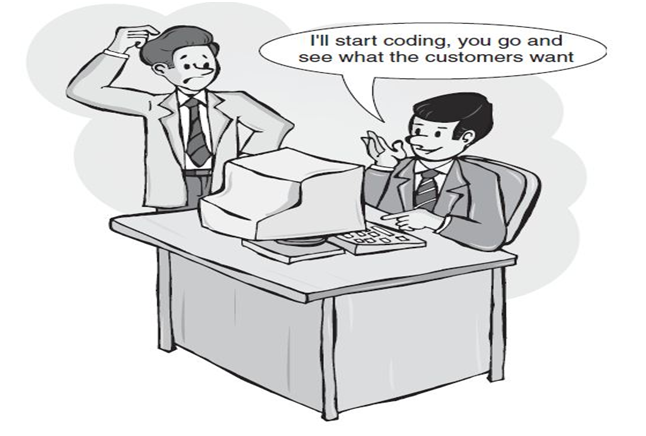
\includegraphics[height=3.5 in]{4-0}
}
\caption{System Requirements}
\label{fg:4-0}
\end{center}
\end{figure}

\begin{figure}
\begin{center}
\fbox{
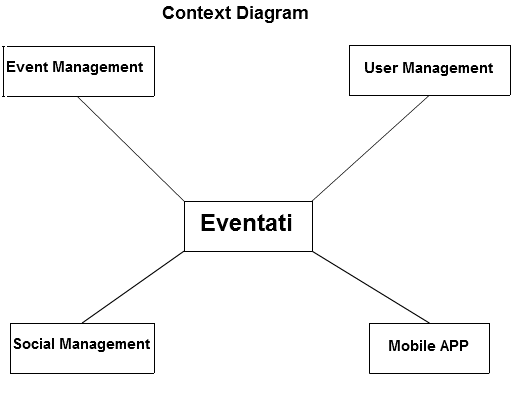
\includegraphics[height=2.5 in]{4-1}
}
\caption{Context Diagram}
\label{fg:4-1}
\end{center}
\end{figure}

\begin{figure}
\begin{center}
\fbox{
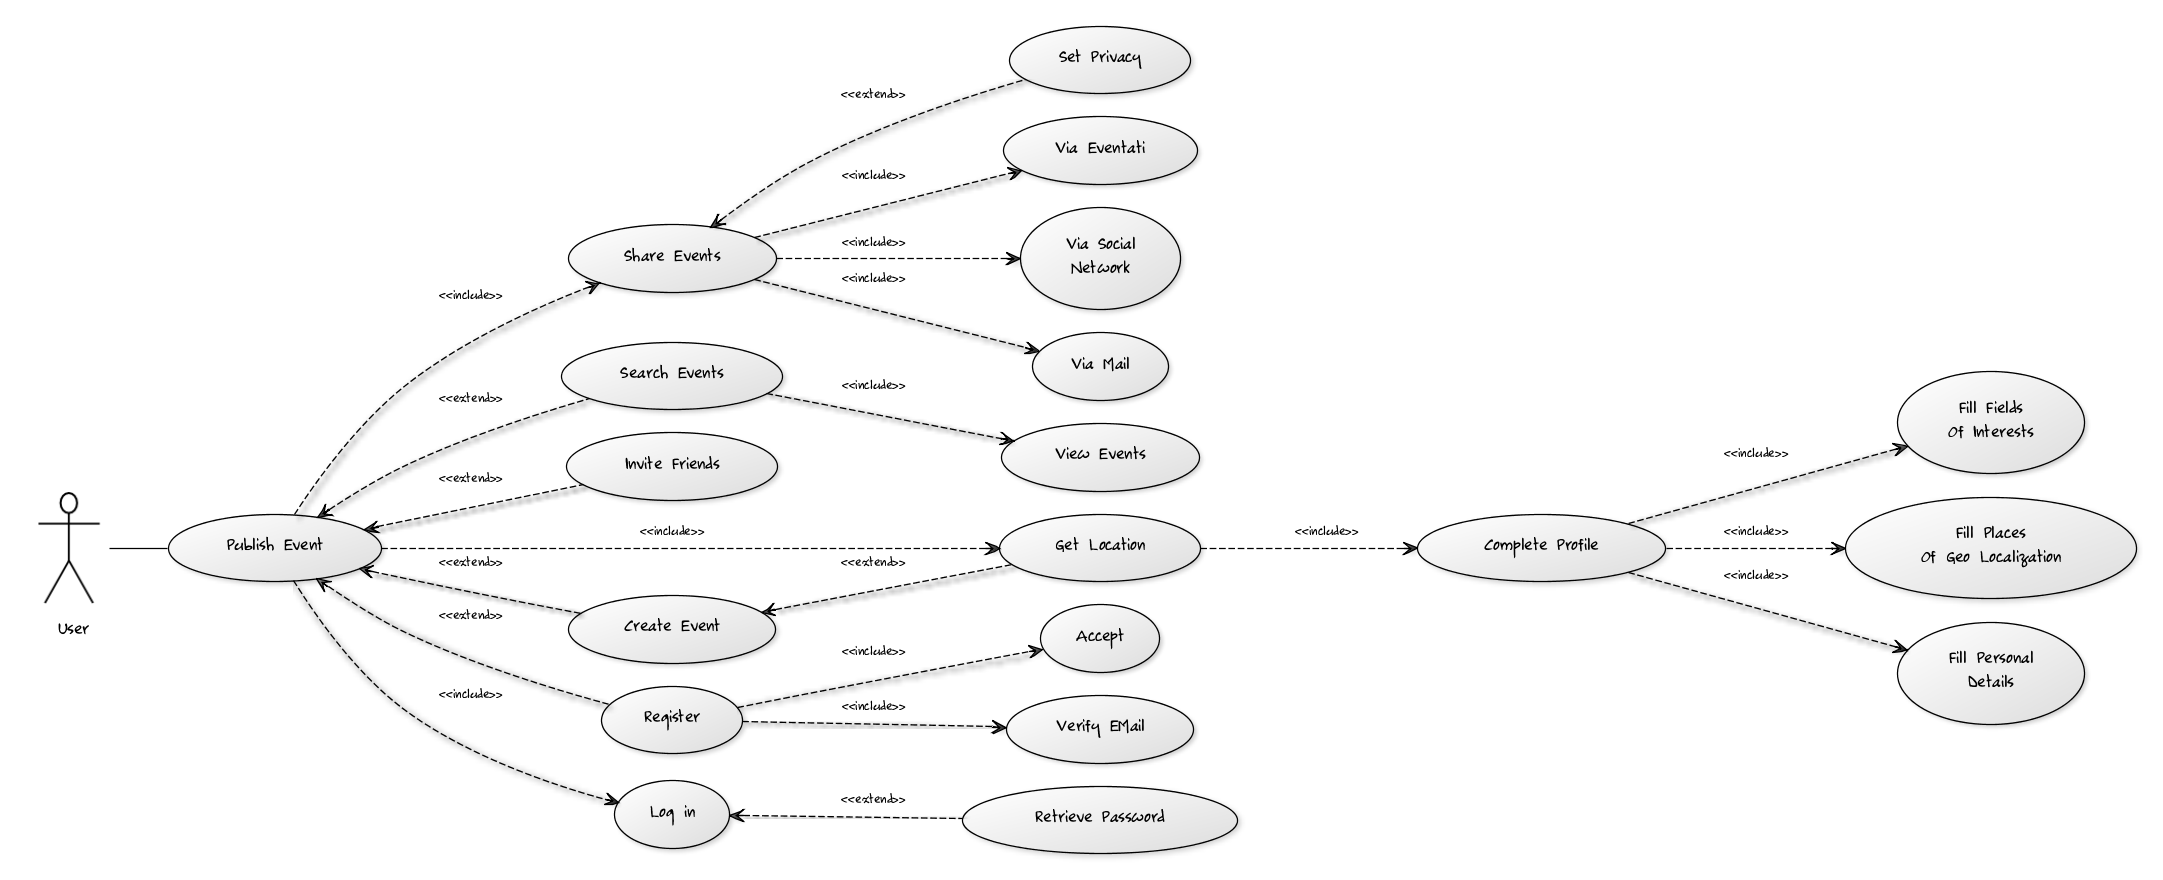
\includegraphics[angle=90,width=3.5 in]{4-2}
}
\caption{Web-UseCase-PublishEvent}
\label{fg:4-2}
\end{center}
\end{figure}
Table 4-1 description Of Publish Events.
\begin{table}
\centering
\begin{tabular}{|l| p{10 cm} |}
\hline
Actor & User (Authorized People) \\ \hline
Description & An Authorized People can publish events via mail, Social Networks or "Eventati: ,Create Events, Search Events, Get Localization and invite Friends .\\ \hline
Data & Event's Attributes .\\ \hline
Stimulus & The Authorized send the data. \\ \hline
Response & Confirmation of the event has been published .\\ \hline
Comments & User must be authorized to make this process.\\ \hline
\end{tabular}
\caption{ Description of Publish Event Process}
\label{tab:table 4-1}
\end{table}

Figure \ref{fg:4-3} presented in page \pageref{fg:4-3} shows Web-Activity-PublishEvent.
\begin{figure}
\begin{center}
\fbox{
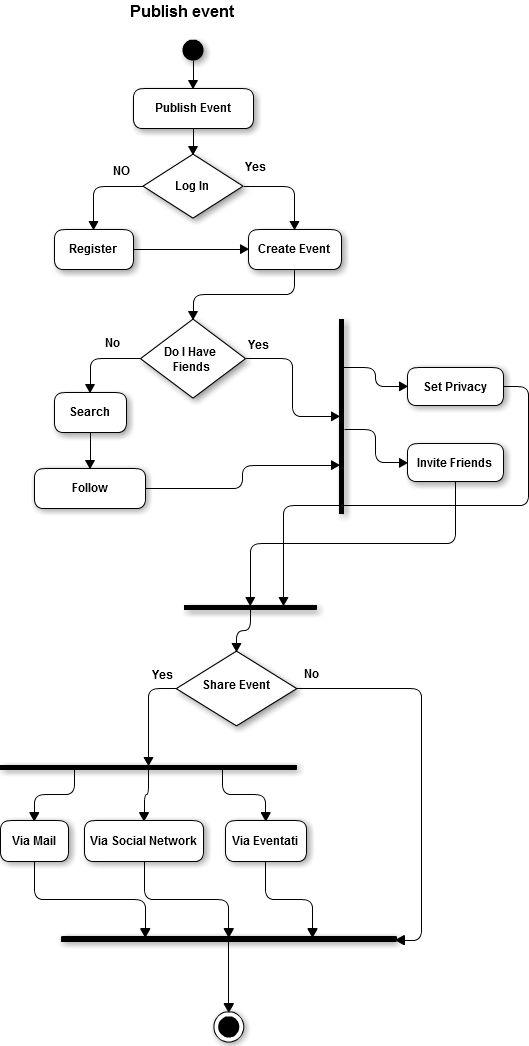
\includegraphics[height=7 in]{4-3}
}
\caption{Web-Activity-PublishEvent}
\label{fg:4-3}
\end{center}
\end{figure}


Figure \ref{fg:4-4} presented in page \pageref{fg:4-4} shows Web-Sequence-PublishEvent.
\begin{figure}
\begin{center}
\fbox{
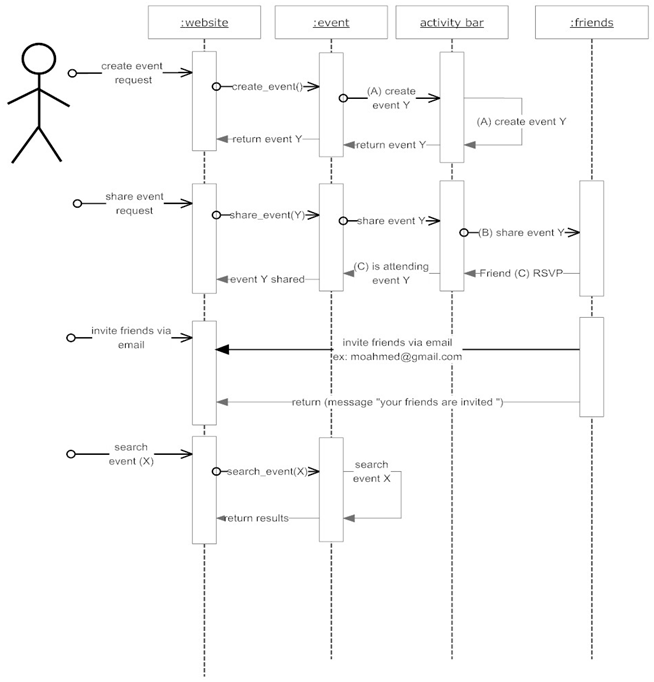
\includegraphics[height=7 in,width=4 in]{4-4}
}
\caption{Web-Sequence-PublishEvent}
\label{fg:4-4}
\end{center}
\end{figure}
\subsection{Find My friends}
\paragraph*{\hspace{.9 cm} } After the previous process system will recommend friends for you if you want and this process is an optional on the system and you can consider it non-functional requirement of the system, another process of our system it is search that is very important process that system must do for the user (functional requirement of the system) search will on event and friends on the system.
Also systems enable us to manage our account such as set privacy, change password and add phone number see. Find friend is one of most important activity for user on system it is available only for authenticated user who only can make this process.
Figure \ref{fg:4-5} presented in page \pageref{fg:4-5} shows Web-Use Case-Find My Friends
\begin{figure}
\begin{center}
\fbox{
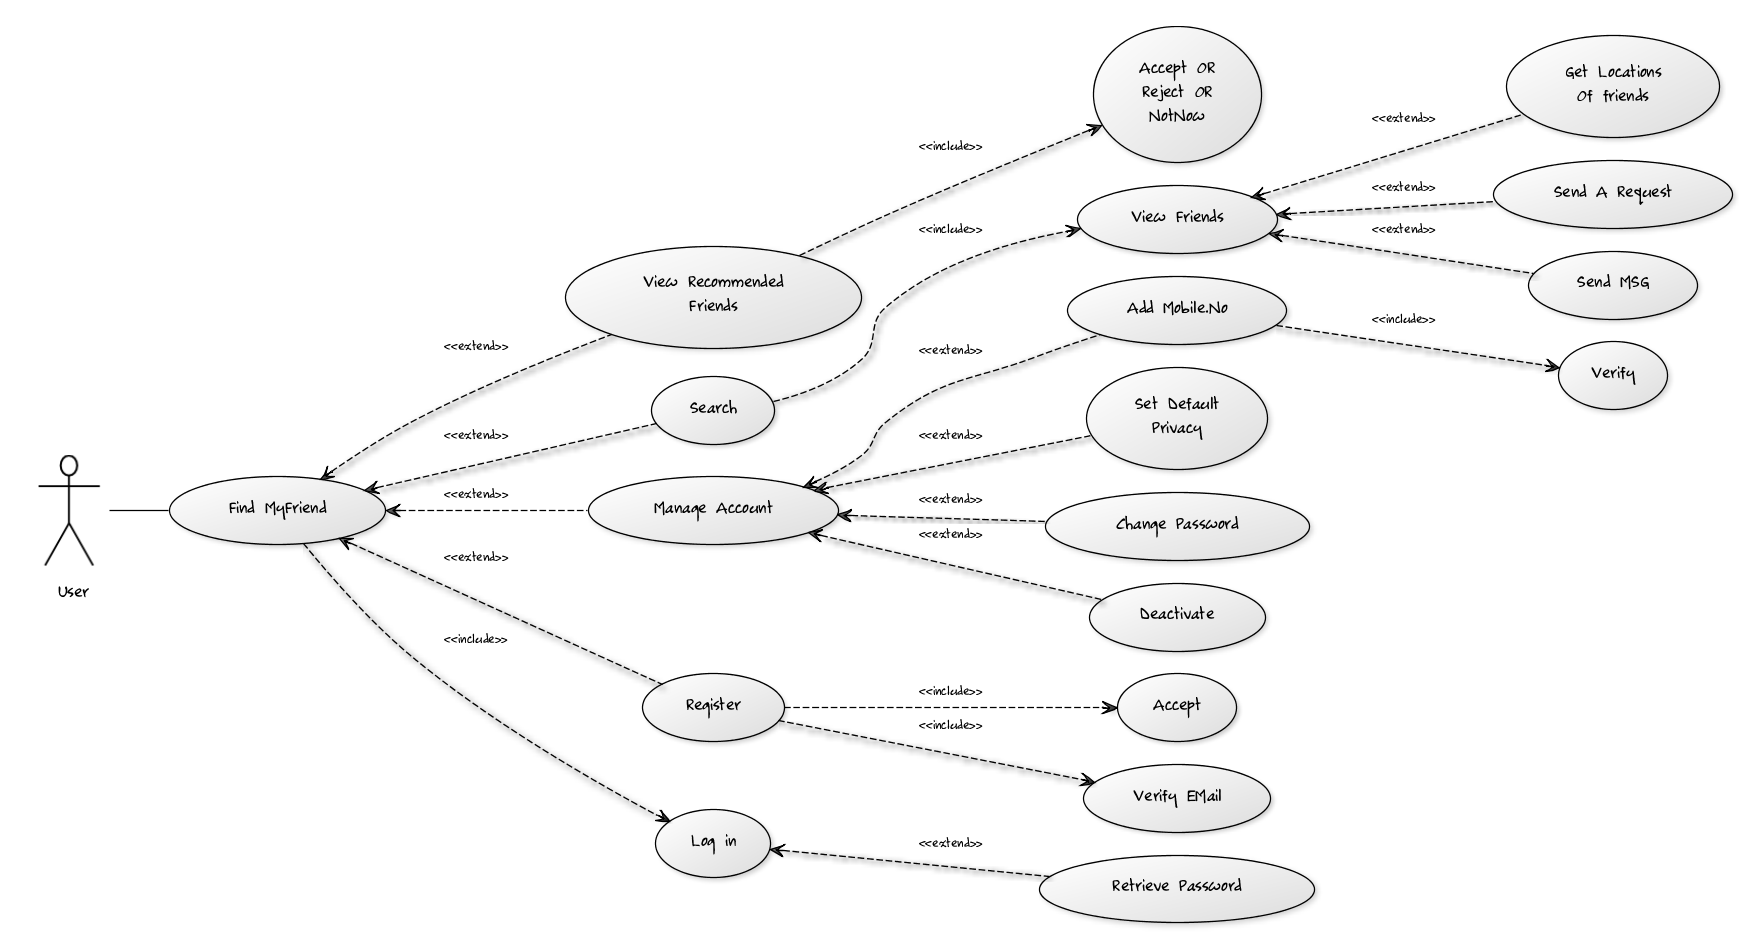
\includegraphics[width=6.5 in,angle=90,height=8 in]{4-5}
}
\caption{Web-Use Case-Find My Friends}
\label{fg:4-5}
\end{center}
\end{figure}
Table 4-2 shows description Of Find My friends Process .And
\begin{table}
\centering
\begin{tabular}{|l| p{10 cm} |}
\hline
Actor & User (Authorized People)and System \\ \hline
Description & An Authorized user can rate, leave a comment and confirm attending with RSVP to  an event 
By Contrast System can notify all subscribes those happened, can also recommend events, friends, places and other activities that appear all in time line.\\ \hline
Data & Information that makes time line be updated or changed. \\ \hline
Stimulus & User command issued by authorized people and system . \\ \hline
Response & Confirmation or changing that happens on-line .\\ \hline
Comments & System must integrate with authorized user.\\ \hline
\end{tabular}
\caption{ Description of Find My Friends Process}
\label{tab:table 4-2}
\end{table}

Figure \ref{fg:4-6} presented in page \pageref{fg:4-6} shows Web-Activity-Find My Friends.
\begin{figure}
\begin{center}
\fbox{
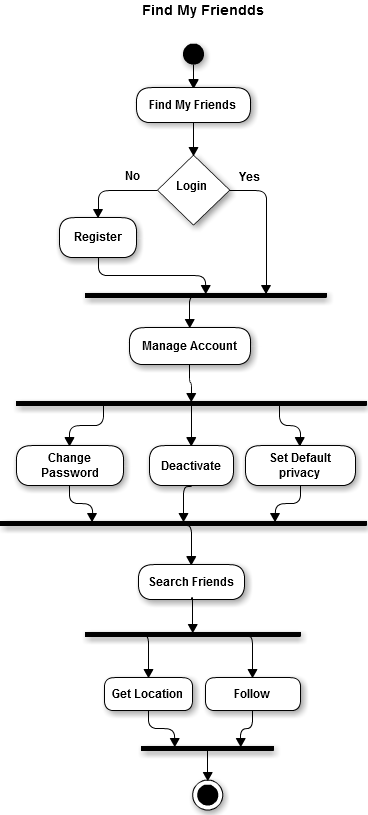
\includegraphics[height=7 in]{4-6}
}
\caption{Web-Activity-Find My Friends}
\label{fg:4-6}
\end{center}
\end{figure}
Figure \ref{fg:4-7} presented in page \pageref{fg:4-7} shows Web-Sequence-Find My Friends
\begin{figure}
\begin{center}
\fbox{
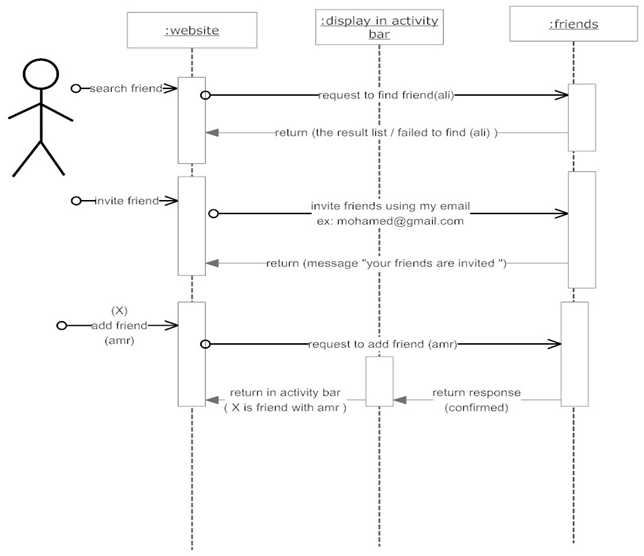
\includegraphics[width=4 in,height=7 in]{4-7}
}
\caption{Web-Sequence-Find My Friends}
\label{fg:4-7}
\end{center}
\end{figure}
\subsection{Update TimeLine}
\paragraph*{\hspace{.9 cm} } System can also make other functional requirements such as system update time line and it must be notified all users about last updates.
It can also recommend activates, places for subscribers and also events. update time line such as confirmed attending via RSVP,left comments on events and rated events.
Also system should provide some assurance technique for user to retrieve any personal data lost on system such as (password).
Figure \ref{fg:4-8} presented in page \pageref{fg:4-8} shows Web-Use Case-Update TimeLine
\begin{figure}
\begin{center}
\fbox{
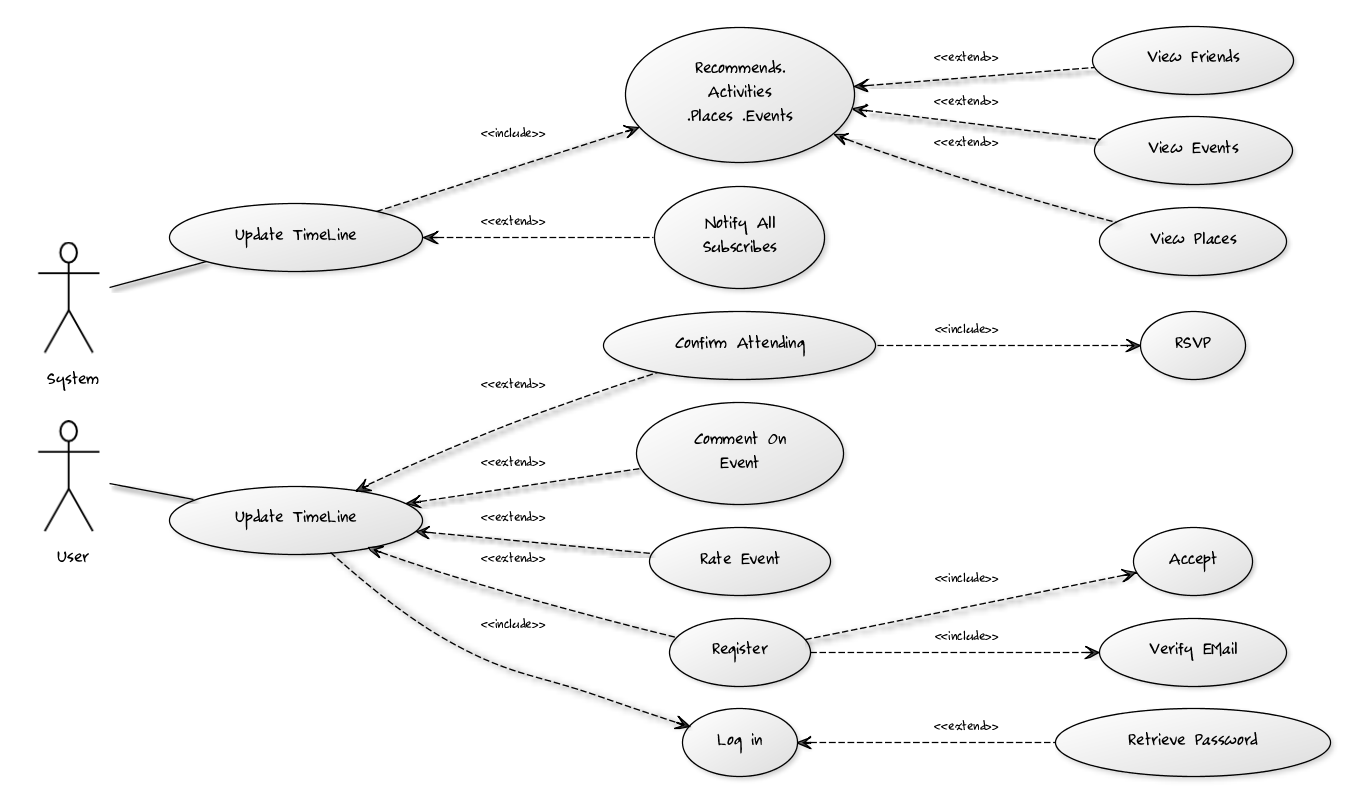
\includegraphics[width=6.5 in,angle=90,height=8 in]{4-8}
}
\caption{Web-Use Case-Update TimeLine}
\label{fg:4-8}
\end{center}
\end{figure}
Table 4-3 description Of Update Time Line
\begin{table}
\centering
\begin{tabular}{|l| p{10 cm} |}
\hline
Actor & User (Authorized People)and System \\ \hline
Description & Users need friends to communicate with each other, so s/he can search and find friends by mail and send them a request for adding. Users can also edit his/her profile.\\ \hline
Data & Requests for friendship send to each other. \\ \hline
Stimulus &User command issued by authorized people . \\ \hline
Response & Users receive accepting or rejecting. \\ \hline
Comments & User must be authorized to make this process, he/she can get location of his/her friends.\\ \hline
\end{tabular}
\caption{ Description of Update TimeLine}
\label{tab:table 4-3}
\end{table}
Figure \ref{fg:4-9} presented in page \pageref{fg:4-9} shows Web-Activity-Update TimeLine
\begin{figure}
\begin{center}
\fbox{
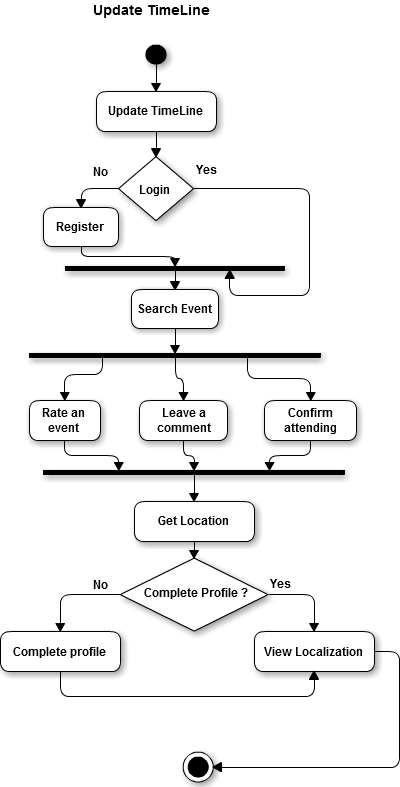
\includegraphics[height=7 in]{4-9}
}
\caption{Web-Activity-Update TimeLine}
\label{fg:4-9}
\end{center}
\end{figure}
Figure \ref{fg:4-10} presented in page \pageref{fg:4-10} shows Web-Sequence-Update TimeLine
\begin{figure}
\begin{center}
\fbox{
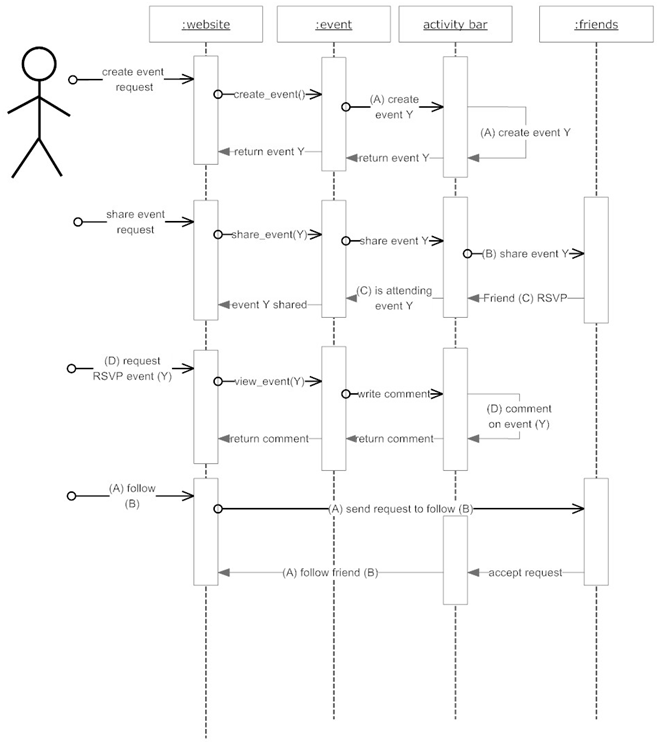
\includegraphics[height=7 in,width=4 in]{4-10}
}
\caption{Web-Sequence-Update TimeLine}
\label{fg:4-10}
\end{center}
\end{figure}
\section{website back-end design}
\paragraph*{\hspace{.9 cm} } One of the important levels of web application implementation is back-end design, it represents dealing with Database including creating, deleting, modifying, and retrieving data, in this project because of depending on Django framework for implementing the web application which is automatically integrate with SQLite database, we need first to design the database by designing Class Diagram Figure \ref{fg:4-11} presented in page \pageref{fg:4-11}shows Class Diagram 
\begin{figure}
\begin{center}
\fbox{
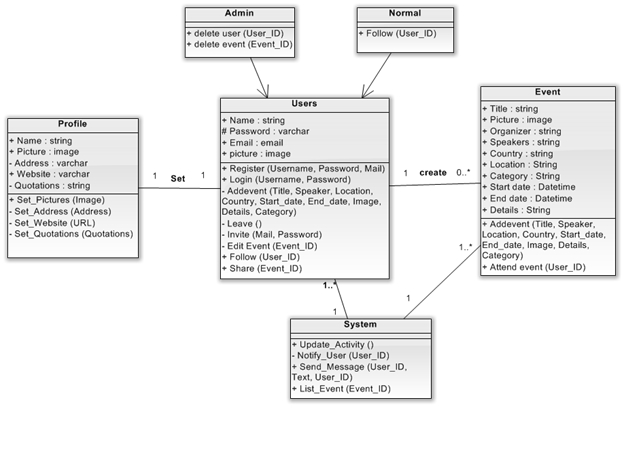
\includegraphics[height=4 in,angle=90,width=6 in]{4-11}
}
\caption{Class Diagram}
\label{fg:4-11}
\end{center}
\end{figure}
and Figure \ref{fg:4-12}  presented in page \pageref{fg:4-12}  shows Entity Relationship
 Diagram "ERD".
 and Figure \ref{fg:4-13}  presented in page \pageref{fg:4-13}  shows  another type Entity Relationship
 Diagram "ERD".
 
\begin{figure}
\begin{center}
\fbox{
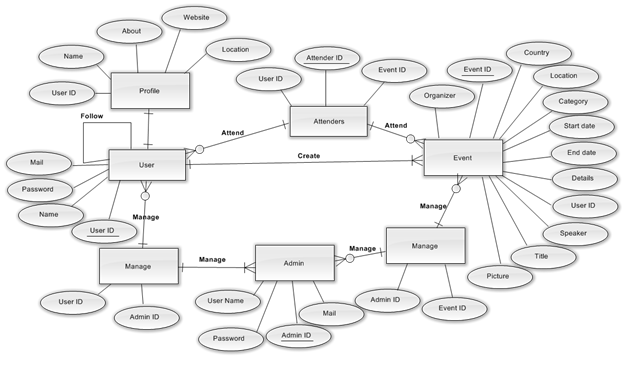
\includegraphics[height=3 in,angle=90,width=4.75 in]{4-12}
}
\caption{Entity Relationship Diagram}
\label{fg:4-12}
\end{center}
\end{figure}
\begin{figure}
\begin{center}
\fbox{
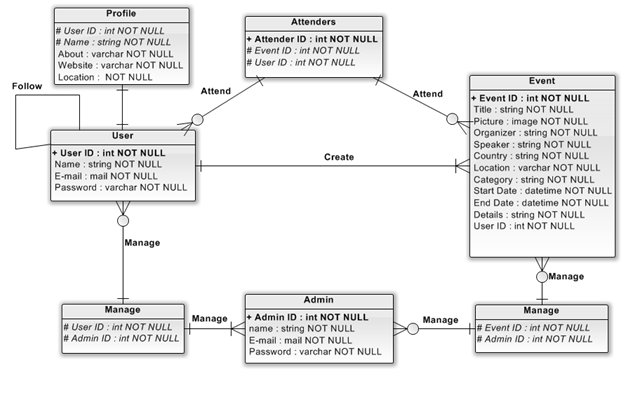
\includegraphics[height=3 in,angle=90,width=5.5 in]{4-13}
}
\caption{Entity Relationship Diagram 2}
\label{fg:4-13}
\end{center}
\end{figure}
Now we can begin to implement the database of the project, in Django you must first create an application by listing this command in the terminal python manage.py startapp application's name it will create an application in your directory then you must insert this application's name in the setting file under the category of installed application after that you can create a table for this application by listing the attributes in the application's model and this is an example of creating table for events which goes as follow in Figure \ref{fg:4-14}  presented in page \pageref{fg:4-14}  shows Application Modeland by a powerful command  python manage.py syncdb it creates a table of entered attributes and automatic generate SQLite commands for this process and this is an example of creating table for events which goes as follow  in Figure \ref{fg:4-15}  presented in page \pageref{fg:4-15}  shows python manage.py syncdb.And after creating tables of database you can import it to the view of the project to apply methods of creating, deleting, and updating data in the database .
\begin{figure}
\begin{center}
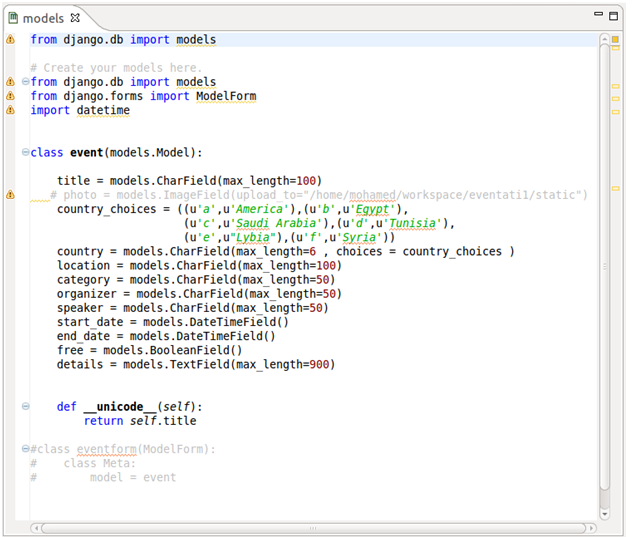
\includegraphics[height=3.5 in]{4-14}
\caption{Application Model}
\label{fg:4-14}
\end{center}
\end{figure}

\begin{figure}
\begin{center}
\fbox{
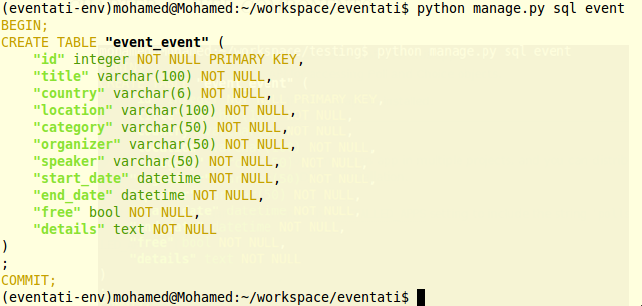
\includegraphics[height=2.5 in]{4-15}
}
\caption{python manage.py syncdb}
\label{fg:4-15}
\end{center}
\end{figure}

\section{Interface Design}
\paragraph*{\hspace{.9 cm} } In this part of the chapter we will talk about pages we have and how they are working, how user accesses them, what is required from the user and how the system manage them and store them then representing them to the user.
 Here are some of that pages we have:
 \begin{itemize}
 \item[•] Landing page.
\item[•] Home page.
\item[•] Create events page.
\item[•]  User's profile page.
\item[•]User setting page.
 \end{itemize}
 \subsection{Landing  page}
\paragraph*{\hspace{.9 cm} }  The first page that the users will see when they visit our site, in which we will find a video to explain our idea for the site and represent it to the users.
In that page there are two things required from the user:
\begin{enumerate}
\item Asking the user to login using his e-mail and password.

\item If the user hasn't registered yet, then ask him to create his own account by filling the registration form which contains the required information (user-name, password, valid e-mail, location), then the user is allowed to access our site.
\end{enumerate}
Figure \ref{fg:4-16} presented in page \pageref{fg:4-16} Here is how the landing page looks like
\begin{figure}
\begin{center}
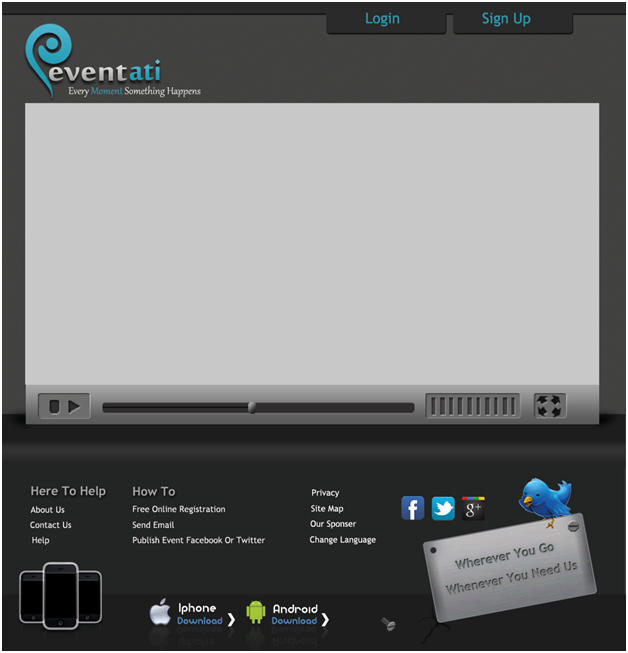
\includegraphics[height=5 in]{4-16}
\caption{Landing Page}
\label{fg:4-16}
\end{center}
\end{figure}
\subsection{Home page}
\paragraph*{\hspace{.9 cm} } The first page that the user will see after logging in, in which there will be   the upcoming events, most recent events, the categories by which we can make finding your interested events easier and more effective. We also find the activity bar that shows you your friends activities, what they share, what they attend and their comments, so it can also be given comments and to be aware of all updates happening around you every second.
  Map, by which system can detect your current location and show you the events around your area.Map not only shows events around you, but also allows you to determine the location of the event you will create or attend.
Here is an example for the most recent events:
\\
Example 1:
Here is the method we use to request the last 5 events recently added by users to be viewed at the top.
Figure \ref{fg:4-17} presented in page \pageref{fg:4-17}
\begin{figure}
\begin{center}
\fbox{
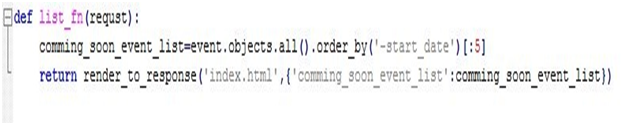
\includegraphics[height=1 in]{4-17}
}
\caption{Example Code Of last 5 Events}
\label{fg:4-17}
\end{center}
\end{figure}
And now it's the calling function to be added the page and specify a space for it in the database
Figure \ref{fg:4-18} presented in page \pageref{fg:4-18} shows code of calling function.
\begin{figure}
\begin{center}
\fbox{
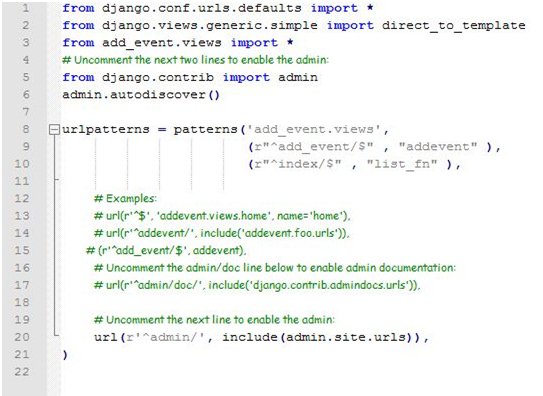
\includegraphics[height=3 in]{4-18}
}
\caption{Code Of Calling Function}
\label{fg:4-18}
\end{center}
\end{figure}
Figure \ref{fg:4-19} presented in page \pageref{fg:4-19} shows The html code for the page
\begin{figure}
\begin{center}
\fbox{
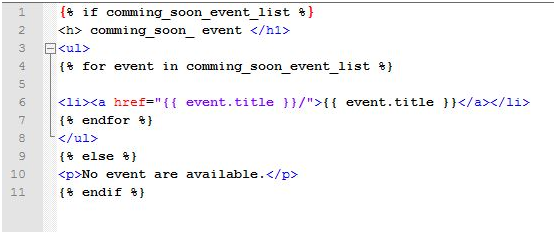
\includegraphics[height=2 in]{4-19}
}
\caption{The html code of page}
\label{fg:4-19}
\end{center}
\end{figure}
Figure \ref{fg:4-20} presented in page \pageref{fg:4-20} shows the final output.
\begin{figure}
\begin{center}
\fbox{
\includegraphics[height=1.25 in]{4-20}
}
\caption{The final output}
\label{fg:4-20}
\end{center}
\end{figure}
\subsection{Create Events}
\paragraph*{\hspace{.9 cm} } Create event, by which the user or the company has the ability to create his own event. In this page there are some fields required from the user:
\begin{itemize}

\item[•] Event name.
\item[•] Photo for the event.
\item[•] Country.
\item[•] Location.
\item[•] Set event's location on the map.
\item[•] Starting and ending date.
\end{itemize}
  	And many other details required about the event.
	We receive the entered information and then it is stored in the database to be represented to the user. We create a model by which we make the initial design or interface of the page and its contents. Then we create a method to call the information entered by the user to save them in the database and return the page to the user.
Figure \ref{fg:4-21} presented in page \pageref{fg:4-21} shows Example 1 Of Create event and
Figure \ref{fg:4-22} presented in page \pageref{fg:4-22} shows Example 2 Of Create event.The previous example represents the method that we use to call the information the user has entered , and now we will show another example that shows us the method that make the fields in which the user will write the information required from them.
\begin{figure}
\begin{center}
\includegraphics[height=3.5 in]{4-21}
\caption{Code 1 Of create Event}
\label{fg:4-21}
\end{center}
\end{figure}
\begin{figure}
\begin{center}
\includegraphics[height=3 in]{4-22}
\caption{Code 2 Of create Event}
\label{fg:4-22}
\end{center}
\end{figure}
The Figure \ref{fg:4-23} presented in page \pageref{fg:4-23} shows the result output. 
\begin{figure}
\begin{center}
\fbox{
\includegraphics[height=2.5 in]{4-23}}
\caption{ The Result Out Put }
\label{fg:4-23}
\end{center}
\end{figure}
\subsection{ Profile Page}
Figure \ref{fg:4-24} presented in page \pageref{fg:4-24} shows The user's profile page is built in the pinax and here is the html code for the page to get the values from the user:
\begin{figure}
\begin{center}
\fbox{
\includegraphics[height=2.5 in]{4-24}
}
\caption{ Code Of user's Profile }
\label{fg:4-24}
\end{center}
\end{figure} 
Figure \ref{fg:4-25} presented in page \pageref{fg:4-25} Shows the page as the following.
\begin{figure}
\begin{center}
\includegraphics[height=4 in]{4-25}
\caption{ user's profile Page }
\label{fg:4-25}
\end{center}
\end{figure}  
\subsection{Setting Page}
Figure \ref{fg:4-26} presented in page \pageref{fg:4-26} Shows The page in which user can control the account, the privacy setting and it's also a built in page in pinax.
\begin{figure}
\begin{center}
\fbox{
\includegraphics[height=2.75 in]{4-26}
}
\caption{ user's profile Page }
\label{fg:4-26}
\end{center}
\end{figure}
\section{Implementation of testing}
\subsection{Testing}
\paragraph*{\hspace{.9 cm} } Automated testing is an extremely useful bug-killing tool for the modern Web developer. You can use a collection of tests to solve, or avoid, a number of problems:
\begin{itemize}

\item[•] When you're writing new code, you can use tests to validate your code works as expected.
\item[•] When you're re-factoring or modifying old code, you can use tests to ensure your changes haven't affected your application's behaviour unexpectedly.
\end{itemize}
\subsection{Why testing ?}
\paragraph*{\hspace{.9 cm} } "Code without tests is broken by design." - Jacob.
Providing automated tests for your code is a way to repeatedly ensure, with minimal developer effort, that the code you wrote to handle a task works as advertised. I like to think of tests as my insurance policy. They generally keep me from breaking existing code and looking foolish to other people. They're also concrete proof that the code works correctly. Without that proof, what you have is a pile of code that worked right once on your machine and that you'll either have to hand-test again and again in the future or will break without you knowing any wiser.
When you first get started, writing tests is a scary task that sounds like extra work. But simple tests are easy to write and having some tests is better than no tests at all. And as you add new tests, your suite (and your confidence) grows with it.
This is not to say that tests solve everything. There will always be bugs in software. Maybe the tests miss a code-path or a user will use something in an unexpected way. But tests give you better confidence and a safety net.
\subsection{When testing? }
\paragraph*{\hspace{.9 cm} } Another point of decision is deciding whether to do \textbf{test-first} (a.k.a. Test Driven Development) or test-after. \emph{Test-first} is where you write the necessary tests to demonstrate proper behaviour of the code \textbf{BEFORE} you write the code to solve the problem at hand. \textbf{Test-after} is when you've already written the code to solve the problem, then you go back and create tests to make sure the behaviour of the code you wrote is correct.
\subsection{Writing testing}
\paragraph*{\hspace{.9 cm} } With Django (and Python in general) there are two main ways to write tests for your projects test suite, doctests and unit tests.
Doctests are written in Python docstrings and unit test are defined with classes.
firstly, - Unit tests – tests that are expressed as methods on a Python class that subclasses unittest.TestCase or Django’s customized TestCase. that helps in "Eventati" and we will show that later.

For a given Django application, the test runner looks for unit tests in two places:
\begin{itemize}
\item[•]The models.py file. The test runner looks for any subclass of unit-test.TestCase in this module.
\item[•] A file called tests.py in the application directory – i.e., the directory that holds models.py. Again, the test runner looks for any subclass of unit-test.TestCase in this module.
\end{itemize}
  
Secondly,- Doctests – tests that are embedded in your functions's docstrings and are written in a way that emulates a session of the Python interactive interpreter. A docstring is a string literal that occurs as the first statement in a module, function, class, or method definition
Figure \ref{fg:4-27} presented in page \pageref{fg:4-27} Shows The Example of Docstrings
\begin{figure}
\begin{center}
\fbox{
\includegraphics[height=.5 in]{4-27}
}
\caption{ Docstrings }
\label{fg:4-27}
\end{center}
\end{figure}
As with unit tests, for a given Django application, the test runner looks for doctests in two places:
\begin{itemize}
\item[•]The models.py file. You can define module-level doctests and/or a doctest for individual models.
\item[•] A file called tests.py in the application directory – i.e., the directory that holds models.py. This file is a hook for any and all doctests you want to write that aren't necessarily related to models. 
This example doctest is equivalent to the example given in the unit-test .
\end{itemize}
\subsection{Handelling Testing Of Eventati}
\paragraph*{\hspace{.9 cm} } Testing a Web application is a complex task, because a Web application is made of several layers of logic – from HTTP-level request handling, to form validation and processing, to template rendering.But we ensure that we must test our code in "Eventati" so we stick to unit-test. This is because tests written in unit-test run the fastest when testing Django applications and this an example of testing events view function .And to run testing write in the shell ( python manage.py test event) .
\cleardoublepage
\chapter{Mobile Components}
\section{ Introduction:}
 \paragraph*{\hspace{.9 cm} } Mobile devices are in widely used especially in the 20's century and still in growing. Mobile devices can be Smart phones, IOS, android, Black Berry, Symbian OS, Windows Phone OS and tablets. Mobile applications are compact software programs that perform specific tasks for the mobile user. It is much easier for the mobile users to conceptualize what this means in practice with the download application on their devices and access it. statistically ,There is 4 billion phones are in use and 1.08 billion are smart phones and as we know mobile applications are applications that run on smart phones or other mobile devices . That is no surprise if we take into account that 5 billion applications were downloaded in 2010. There are some serious predictions that 21 billion applications will be downloaded by 2013.\\
  Everything could be done via mobile applications, to simplify your work and life you'll likely want to find applications that will help you keep up with social networking and stay productive while on the go. The growth in mobile technologies has meant that businesses in certain sectors are even receiving most of their web traffic from users browsing in mobile devices.
 \\ The numbers of mobile users in Egypt reach to 72.94 million in February 2011, increasing from 71.50 Million in January 2011. Number of Mobile subscribers in February 2010 was 56, 49 Million subscribers [ Elwaset]. With the increase in mobile subscribers in Egypt, it becomes important to target those users.
So appcelerator titanium that we used to build the application.
\section{User Requirements:}
\subsection{Update TimeLine}
 \paragraph*{\hspace{.9 cm} } User requirements of mobile application that means "Use Case Diagram".  In each Project we must determine requirements of users that specify the requirements the user expects from software to be constructed in a software projects. To extract it we analysis the system and represent it in a use case Diagram showing in figure 5.1 have been drawn by using this tool "Website" http://yuml.me/  and the described table in table 5.1 in the below. 
 Figure \ref{fg:5-1} presented in page \pageref{fg:5-1}shows Mobile-Use Case-Update TimeLine
\begin{figure}
\begin{center}
\fbox{
\includegraphics[width=6.5 in,angle=90,height=8 in]{5-1}
}
\caption{Mobile-Use Case-Update TimeLine}
\label{fg:5-1}
\end{center}
\end{figure}
Table 5-1 description Of Update Time Line
\begin{table}
\centering
\begin{tabular}{|l| p{10 cm} |}
\hline
Actor & User (Authorized People). \\ \hline
Description & An Authorized user can rate, leave a comment and confirm attending with RSVP to an event, find friends, Search events, create events by web view and view all events.\\ \hline
Data & Information that makes time line be updated or changed . \\ \hline
Stimulus & User command issued by authorized people and system . \\ \hline
Response & Confirmation or changing that happens on-line . \\ \hline
Comments & System must integrate with authorized user.\\ \hline
\end{tabular}
\caption{ Description of Update TimeLine For Mobile}
\label{tab:table 5-1}
\end{table}
Definitely, we have many processes in our application but we prefer to collect all of them in the main processes, since our application is simple we found only one primary process is "updating time line".
To update Time line we must be logged to the application but, if we're not registered, we should register to the Application to access functions of the application. After logging, you can perform your processes, you can search and view events that will be executed or done, then you decide if you want to attend or not through RSVP, then you can invite your friends and share them with each other. If you notice the importance the events you will attend you can rate them to give a feedback, or if you have a comment you can leave it. You can't only attend events but also you can create events with its attributes, if you want to announce it and determine the place of its location through a web view. You can also send requests to adding friends to communicate and share events with each others.
\section{User Interaction with Mobile application:}
\paragraph*{\hspace{.9 cm} } User interaction with mobile applications means "Activity Diagram". In an activity diagram is a simple and intuitive illustration of what happens in a work-flow, what activities can be done in parallel, and whether there are alternative paths through the work-flow. Activity Diagram can be used to describe the operations step-by-step work-flows of components in a system. An activity diagram shows the overall flow of control. Interaction with our application is very simple not complicated at all. Figure \ref{fg:5-2} presented in page \pageref{fg:5-2}shows Mobile-Activity-Update TimeLine.
Activity Diagram in "Eventati" mobile application goes as follows: 
\begin{itemize}
\item[•]We first check connection, login and local file xml to start performing processes in our application, if it is yes or it is not No.
\item[•]If yes there is a connection we have another condition of login if yes login and has a local file xml, now authorized users can perform process.
\item[•] But if it isn't logged they must register to the application.
\item[•] If there is not a connection and a local xml file less than 1 day then alert that to the user, if not then install a new xml file from the web.
\item[•] After that we can search or create events through web view, then we can rate event, confirm attending, leave comments and invite Friends, then you can get location but after your complete profile.
\end{itemize}

\begin{figure}
\begin{center}
\fbox{
\includegraphics[height=7 in]{5-2}
}
\caption{Mobile-Activity-Update TimeLine}
\label{fg:5-2}
\end{center}
\end{figure}
\section{Code of Mobile Application}
 \paragraph*{\hspace{.9 cm} } "Eventati" mobile application has been developed by using Appcelerator Titanium with java script to build native mobile application and to create a version of the application for each targeted device. "Eventati" mobile application has been applied to android and I Phone OS also with the same code. 
Here, is a copy of an example code that we worked on it:
first,
Figure \ref{fg:5-3} presented in page \pageref{fg:5-3}shows Code Of Landing page that contains logo, slogan,Get-started Function ,Learn More which Contains slides of explaining Application
\begin{figure}
\begin{center}
\fbox{
\includegraphics[height=4.75 in]{5-3}
}
\caption{Code of Landing Page}
\label{fg:5-3}
\end{center}
\end{figure}
Second:
Figure \ref{fg:5-4} presented in page \pageref{fg:5-4}shows Code Of Slides that define Application to Any Users.
\begin{figure}
\begin{center}
\fbox{
\includegraphics[height=5 in]{5-4}
}
\caption{Code Of the Slides Images}
\label{fg:5-4}
\end{center}
\end{figure}
Third:
Figure \ref{fg:5-5} presented in page \pageref{fg:5-5}shows Code Of Login Page Which allows users entering to "Eventati "Application.
\begin{figure}
\begin{center}
\fbox{
\includegraphics[height=6.9 in,width=4 in ]{5-5}
}
\caption{Code of Login page}
\label{fg:5-5}
\end{center}
\end{figure}
fourth:
Figure \ref{fg:5-6} presented in page \pageref{fg:5-6}shows Code Of Agenda which contains a list of events will be implemented.
\begin{figure}
\begin{center}
\fbox{
\includegraphics[height=8.5 in]{5-6}
}
\caption{Code of Agenda}
\label{fg:5-6}
\end{center}
\end{figure}
Five:
Figure \ref{fg:5-7} presented in page \pageref{fg:5-7}shows Code Of Event details which contains attributes of each event.
\begin{figure}
\begin{center}
\fbox{
\includegraphics[height=3.5 in]{5-7}
}
\caption{Code Of Event details}
\label{fg:5-7}
\end{center}
\end{figure}
\cleardoublepage
\chapter{Design Components }
\section{Introduction}
\paragraph*{\hspace{.9 cm} }  Web design means to create effective interface between technology and people which allows them to present their information and use it for meaningful purposes. The interface is a fundamental part of making the site more successful, safe, useful, functional , and in the long run more pleasurable for the user.A good website starts life in the design stage. If a website is attractive enough it can attract traffic towards it and the increase in traffic always result in the increase in business. There are several aspects of the site that are formed at this stage, including among other things, layout, color, content, functionality and maintainability.
\section{Logo Design}
\paragraph*{\hspace{.9 cm} } The logo identifies the website via the use of a mark, flag, symbol or signature. A simple logo design allows for easy recognition and allows the logo to be versatile and memorable.In "Eventati", we used “text and symbol logo” by using “map pin” icon which portrays one of the functionalities of the website .The map pin is used to mark points on the map .similarly, "Eventati" gives the users the ability to reach the most important ,famous, popular and exciting events around the world via one click.
There are many stages that we went through to reach the final result:
 Figure \ref{fg:6-1} presented in page \pageref{fg:6-1} shows Every color and AscIICode we Used it. 
Our first try resulted in the logo in Figure \ref{fg:6-2} presented in page \pageref{fg:6-2} in which we used the colors “  f0983f” and “ fafafa   ” and  the font” Lucida Handwriting”. Then, we designed the second logo in Figure \ref{fg:6-3} presented in page \pageref{fg:6-3} in which we used the color "  69b9cb ", and the font "karabinE". Finally, we changed it as we found that it’ll be difficult for the user to read it . The new logo in Figure \ref{fg:6-4} presented in page \pageref{fg:6-4} is simple and to-the-point. The new colors sit much nicer than the old ones as We used  the color ” 9c9e9a”  to present  the word event  and  the  color “37aabe”  for the entire logo and the font  ” MoolBoran” . 
\\
As the slogan is a very important element for a website because it makes it that much easier to increase users retention, rate and desire, we choose a slogan in Figure \ref{fg:6-5} presented in page \pageref{fg:6-5} that represent what we are trying to help the user not to miss.

\begin{figure}
\begin{center}
\includegraphics[height=1.5 in]{6-1}
\caption{AscII Code Colors}
\label{fg:6-1}
\end{center}
\end{figure}
 \begin{figure}[ht]
	\begin{minipage}[b]{0.5\linewidth}
	\centering
	\includegraphics[scale=.6]{6-2}
	\caption{First Logo }
	\label{fg:6-2}
	\end{minipage}
	\hspace{0.5cm}
	\begin{minipage}[b]{0.5\linewidth}
	\centering
	\includegraphics[width=\textwidth]{6-3}
	\caption{Second Logo}
	\label{fg:6-3}
	\end{minipage}
	\end{figure}
 \begin{figure}[ht]
	\begin{minipage}[b]{0.5\linewidth}
	\centering
	\includegraphics[scale=.6]{6-4}
	\caption{Final Logo Of Eventati}
	\label{fg:6-4}
	\end{minipage}
	\hspace{0.5cm}
	\begin{minipage}[b]{0.5\linewidth}
	\centering
	\includegraphics[width=\textwidth]{6-5}
	\caption{Slogan Of Eventati}
	\label{fg:6-5}
	\end{minipage}
	\end{figure}
\section{Web pages layouts}
\subsection{Landing page}
 \paragraph*{\hspace{.9 cm} } Landing page is the first page that the user perceives upon entering the website URL at the browser addresses area.\\
First, we have designed page Figure \ref{fg:6-6} presented in page \pageref{fg:6-6} show initial landing page which contain form for login process, sign up link, and slides how which contain several slides to introduce our project and our services, then we have made some changes, we have exchanged the sign up link with sign up form to facilitate the process of signing up Figure \ref{fg:6-7} presented in page \pageref{fg:6-7} shows Second Landing Page.
Finally we designed an interactive landing page which contains a login form where user-name and password can be entered. A validation is performed to verify whether the user is an already authorized user, if not the user is allowed to sign up by filling up the necessary details on the registration form. Both of login and registration forms are located in Slide Down jQuery, and exchanged the slide show with a video as Videos are one of the best methods for communicating with audiences because it's much easier to consume the visual image than to read something. The visual impact created by videos can often be creatively used to reach out and capture the imagination of a wide audience.The landing page appears as given below Figure \ref{fg:6-8} presented in page \pageref{fg:6-8} shows The final landing page.
 \begin{figure}
	\begin{minipage}[b]{0.5\linewidth}
	\centering
	\includegraphics[height=2.5 in]{6-6}
	\caption{First Logo }
	\label{fg:6-6}
	\end{minipage}
	\hspace{0.5cm}
	\begin{minipage}[b]{0.5\linewidth}
	\centering
	\includegraphics[width=\textwidth]{6-7}
	\caption{Second Logo}
	\label{fg:6-7}
	\end{minipage}
	\end{figure}
\begin{figure}
\begin{center}
\includegraphics[height=5.5 in]{6-8}
\caption{Final landing Page}
\label{fg:6-8}
\end{center}
\end{figure}
\subsection{Home page}
 \paragraph*{\hspace{.9 cm} }The home page Figure \ref{fg:6-9} presented in page \pageref{fg:6-9} shows the Home page of "Eventati" website is the first page that appears to the user after a successful login. The entire website depends on how the home page is designed which forms the platform for viewing other web forms. In short, the home page form is the abstract of the entire website. On home page you can review upcoming events ordered by date of creation or number of views. TimeLine exists to show current events and friends activities ordered by date when it was made, tag cloud which provide visitors with an instant illustration of the most important and popular subjects in the site dynamically.
\begin{figure}
\begin{center}
\includegraphics[height=8 in]{6-9}
\caption{Eventati  Home Page}
\label{fg:6-9}
\end{center}
\end{figure}
\subsection{Create event page}
This page supports creating events, you'll be asked to input your event's name and location, as well as a start and end time, and some additional information about your events as shown in Figure \ref{fg:6-10} presented in page \pageref{fg:6-10} shows Home Page of "Eventati".
\begin{figure}
\begin{center}
\includegraphics[height=8.10 in]{6-10}
\caption{Create events Page}
\label{fg:6-10}
\end{center}
\end{figure}
\subsection{Profile page }
 \paragraph*{\hspace{.9 cm} } Profile page Figure \ref{fg:6-11} presented in page \pageref{fg:6-11} is the personal community page.  Showing photos, friends, some personal information, also Favourites, attended, and created events as well as allows sharing events and invite friends. Profile page can be viewed by logged in users.
 \begin{figure}
\begin{center}
\includegraphics[height=8.10 in]{6-11}
\caption{Profile Page}
\label{fg:6-11}
\end{center}
\end{figure}
\subsection{Event Details page}
 \paragraph*{\hspace{.9 cm} } After clicking on the event, you will receive event details page in Figure \ref{fg:6-12} presented in page \pageref{fg:6-12} in which users can find all details like: event location, start and end date, event organizer, speaker, type, and the additional details about the event. As well as users find comments about the event and can post comments, also find the event latest updates. Users can share and invite guests to the event. The user who created the event can click on the event to view and edit some details about the event.
 
\begin{figure}
\begin{center}
\includegraphics[height=8.10 in]{6-12}
\caption{Event Details page}
\label{fg:6-12}
\end{center}
\end{figure}

\subsection{Search page}
\paragraph*{\hspace{.9 cm} } After typing what the users looking for, s/he will receive advanced search page Figure \ref{fg:6-13} presented in page \pageref{fg:6-13} which contains all results about what s/he searched for. "Eventati" provides search for friends and events. 
\begin{figure}
\begin{center}
\includegraphics[height=8.10 in]{6-13}
\caption{Search page}
\label{fg:6-13}
\end{center}
\end{figure}
\section{Design in Mobile Application}
\paragraph*{\hspace{.9 cm} } Everywhere you turn these days people are talking about mobile applications. Applications for this, applications for that.the mobile application can be used to increase the number of "Eventati" users but mobile application Can't be attractive for users without a Good Design .
\section{Mobile Icons}
\paragraph*{\hspace{.9 cm} } For "Eventati" mobile application we designed "hand drawing icons" in size 32 and 48 pixel as shown in Figure 6.14 presented in page 81 but it didn't fit with the application so we designed another icons as shown in Figure \ref{fg:6-15} presented in page \pageref{fg:6-15}
 \begin{figure}
	\begin{minipage}[b]{0.5\linewidth}
	\centering
	\includegraphics[height=1.20 in]{6-14}
	\caption{Hand Drawing Mobile Icons }
	\label{fg:6-13}
	\end{minipage}
	\hspace{0.5cm}
	\begin{minipage}[b]{0.5\linewidth}
	\centering
	\includegraphics[width=\textwidth]{6-15}
	\caption{Final Mobile Icons}
	\label{fg:6-15}
	\end{minipage}
	\end{figure}
\subsection{Mobile layout}
\paragraph*{\hspace{.9 cm} } Figure \ref{fg:6-16} presented in page \pageref{fg:6-16} shows Meeting that we decided the final layout which will appear when you decide to use "Eventati" mobile application. We used slide show with animated photos to introduce our application and our services, and this is the pages we have used in it. The page in Figure \ref{fg:6-17} presented in page \pageref{fg:6-17} shows  the Land Page. .Figure \ref{fg:6-18} presented in page \pageref{fg:6-18} asks our members to login or became one of our fans by signing up . In this page Figure \ref{fg:6-19} presented in page \pageref{fg:6-19} explains that the application gives the user the ability to create ,attend and share events. Figure \ref{fg:6-20} presented in page \pageref{fg:6-20} shows some of our service, as our users can add friends and customize their profile settings.
\begin{figure}
\begin{center}
\includegraphics[height=4 in,angle=90,width=\textwidth]{6-16}
\caption{Mobile Layout}
\label{fg:6-16}
\end{center}
\end{figure}
 \begin{figure}
	\begin{minipage}[b]{0.5\linewidth}
	\centering
	\includegraphics[height=4 in]{6-17}
	\caption{Landing Page}
     \label{fg:6-17}
	\end{minipage}
	\hspace{0.5cm}
	\begin{minipage}[b]{0.5\linewidth}
	\centering
	\includegraphics[width=\textwidth]{6-18}
	\caption{Slide 1}
	\label{fg:6-18}
	\end{minipage}
	\end{figure}
\begin{figure}
	\begin{minipage}[b]{0.5\linewidth}
	\centering
	\includegraphics[height=4 in]{6-19}
	\caption{Slide 2}
     \label{fg:6-19}
	\end{minipage}
	\hspace{0.5cm}
	\begin{minipage}[b]{0.5\linewidth}
	\centering
	\includegraphics[width=\textwidth]{6-20}
	\caption{Slide 3}
	\label{fg:6-20}
	\end{minipage}
	\end{figure}

\cleardoublepage
\chapter{Integration Between Mobile and web }

\section{Introduction}
\paragraph*{\hspace{.9 cm} } It becomes an urgent need to use mobile applications applications . Users increases their use for mobile phone applications and web applications will become just data warehouse.If we have a look for the (Figure 7.1) we will see how mobile use in U.S increased to become 81 minutes per day for Mobile Applications compared to
74 minutes for web consumptions.
Figure \ref{fg:7-1} presented in page \pageref{fg:7-1}shows the consumption between web and mobile Application. 
\begin{figure}
\begin{center}
\includegraphics[height=2 in]{7-1}
\caption{Web and Mobile consumption per day}
\label{fg:7-1}
\end{center}
\end{figure}
This leads us to the importance of mobile development nowadays and also the integration between mobile and web application instead of web application.
\section{Integration Methods} 
\paragraph*{\hspace{.9 cm} }In our mobile Application we uses the most common integration method between mobile and web Applications which called Mobile Web Service .
The main function of this method is to use the whole Web Application DataBase and the whole  functions of DataBase (Insert , Update , Delete ,Select) to make the useful usage of mobile Application . DB Integration Method have the main advantage of data integrity which make no restrictions of misuse between Mobile user And Web User As all data warehouse is shared in the same place and all kinds of users (Mobile , Web) make the same required functions but in some difference in user interface or data required.	Data required for inserting or selecting in mobile differ from web  with the hope of leading best user usage of Mobile Application , In mobile application we require less data from web .	Our method to use Web Services on mobile Application in XmlRPC method.

\section{XmlRPC}
\subsection{Overview}
\paragraph*{\hspace{.9 cm} } XML-RPC is a Remote Procedure Calling protocol that works over the Internet.
An XML-RPC message is an HTTP-POST request. The body of the request is in XML. A procedure executes on the server and the value it returns is also formatted in XML.
Procedure parameters can be scalars, numbers, strings, dates and can also be complex record and list structures.Figure \ref{fg:7-2} and \ref{fg:7-3} presented in page \pageref{fg:7-2} and \pageref{fg:7-3}.
\begin{figure}
\begin{center}
\includegraphics[height=3.5 in]{7-2}
\caption{"Integration Between Mobile and Web"}
\label{fg:7-2}
\end{center}
\end{figure}

\begin{figure}
\begin{center}
\fbox{
\includegraphics[height=3.5 in]{7-3}
}
\caption{"Xml RPC"}
\label{fg:7-3}
\end{center}
\end{figure}
\subsection{request Example}
\subsection{Header requirements}
  \paragraph*{\hspace{.9 cm} } The format of the URI in the first line of the header is not specified. For example, it could be empty, a single slash, if the server is only handling XML-RPC calls. However, if the server is handling a mix of incoming HTTP requests, we allow the URI to help route the request to the code that handles XML-RPC requests. (In the example, the URI is /RPC2, telling the server to route the request to the "RPC2" responder.)
A User-Agent and Host must be specified. 
The Content-Type is text/xml. 
The Content-Length must be specified and must be correct.
\subsection{Payload format}
\paragraph*{\hspace{.9 cm} } The payload is in XML, a single "methodCall" structure.
The  $<$ methodCall $>$    must contain a $<$methodName$>$ sub-item, a string, containing the name of the method to be called. The string may only contain identifier characters, upper and lower-case A-Z, the numeric characters, 0-9, underscore, dot, colon and slash. It's entirely up to the server to decide how to interpret the characters in a $<$methodName$>$. 
For example, the $<$methodName$>$ could be the name of a file containing a script that executes on an incoming request. It could be the name of a cell in a database table. Or it could be a path to a file contained within a hierarchy of folders and files.
If the procedure call has parameters, the  $<$ methodCall $>$ must contain a $<$params$>$ sub-item. The $<$params$>$ sub-item can contain any number of $<$params$>$, each of which has a $<$value$>$. Figure \ref{fg:7-4} presented in page \pageref{fg:7-4} shows Code of Request Example .
\begin{figure}
\begin{center}
\fbox{
\includegraphics[height=2.5 in]{7-4}
}
\caption{"Request Example Code "}
\label{fg:7-4}
\end{center}
\end{figure}
\subsection{Response format}
Unless there's a lower-level error, always return 200 OK.
The Content-Type is text/xml. Content-Length must be present and correct.
The body of the response is a single XML structure, a $<$methodResponse$>$, which can contain a single $<$params$>$ which contains a single $<$params$>$ which contains a single $<$value$>$.
The $<$methodResponse$>$ could also contain a $<$fault$>$ which contains a $<$value$>$ which is a $<$struct$>$ containing two elements, one named $<$faultCode$>$, an $<$int$>$ and one named $<$faultString$>$, a $<$string$>$.
A $<$methodResponse$>$ can not contain both a $<$fault$>$ and a $<$params$>$.
\subsection{Response Example}
\paragraph*{\hspace{.9 cm} } Here's an example of a response to an XML-RPC request.Figure \ref{fg:7-5} presented in page \pageref{fg:7-5} shows Response Code Example "Eventati" .
\begin{figure}
\begin{center}
\fbox{
\includegraphics[height=2.5 in]{7-5}
}
\caption{"Response Code Example  "}
\label{fg:7-5}
\end{center}
\end{figure}

\section{Code Examples:}
\subsection{Example from Xml File:}
Here is code examples from our work in "Eventati" Mobile Application.Figure \ref{fg:7-6} presented in page \pageref{fg:7-6} shows Code Example of "Eventati" .
\begin{figure}
\begin{center}
\fbox{
\includegraphics[height=2.5 in]{7-6}
}
\caption{"Code Example  "}
\label{fg:7-6}
\end{center}
\end{figure}
 
\subsection{Example From UI Application Files}
 \paragraph*{\hspace{.9 cm} }	Example From UI Application Files of reading data from local Xml File After Downloading It from the website :
 	Figure \ref{fg:7-7} presented in page \pageref{fg:7-7} shows UI Application File .
\begin{figure}
\begin{center}
\fbox{
\includegraphics[scale=.63]{7-7}
}
\caption{"UI Application File "}
\label{fg:7-7}
\end{center}
\end{figure}
Figure \ref{fg:7-8} presented in page \pageref{fg:7-8} shows UI Application File2 .
\begin{figure}
\begin{center}
\fbox{
\includegraphics[height=3.5 in]{7-8}
}
\caption{"UI Application File2 "}
\label{fg:7-8}
\end{center}
\end{figure}
Click Hand Function : Is A function occurs when user click on an event to show the event Details :
Figure \ref{fg:7-8} presented in page \pageref{fg:7-9} shows Event Details Code .
\begin{figure}
\begin{center}
\fbox{
\includegraphics[height=3.5 in]{7-9}
}
\caption{Event Details Code}
\label{fg:7-9}
\end{center}
\end{figure}
\cleardoublepage
 \chapter{Outcomes}

\section{Web Outcome}
\begin{itemize}
\item
Figure \ref{fg:8-1} presented in page \pageref{fg:8-1} shows The Land page of"Eventati" the numbers on this figure shows:
\begin{enumerate}
\item Number 1:Shows the Video which explains and presents functions and what "Eventati" will present to users.
\item Number 2 : Shows Login which we can login to "Eventati" by Authorized Users and passwords 
\item Number 3:Shows SignUp which any one can register to "Eventati" by UserName ,e-mail and Password.
\item Number 4 :Shows Logo and Slogan of "Eventati" 
and Finally at the end of each page contains footer which contains fast links to reach the process.
\end{enumerate}
\item Figure \ref{fg:8-17} presented in page \pageref{fg:8-17} shows the land page after Pressing Login Button.
\item Figure \ref{fg:8-18} presented in page \pageref{fg:8-18}shows the land page after Pressing Registration Button.
\item Figure \ref{fg:8-2} presented in page \pageref{fg:8-2} shows shows The Home Page of "Eventati" the numbers on this figure shows:
\begin{enumerate}
\item Number 1 : Shows the Map which contains bins and location of each event.
\item Number 2 : Shows the button which can click and create event.
\item Number 3 : shows events both Most popular and which recently add.
\item Number 4 : Shows Activities or Time Line updating that shows Authorized users activities like (Confirm Attending,Rate Event,Publish Event,leave comments on Events ). 
\item Number 5 : Shows popular tags which contains all categories of events that we interested  in .
\end{enumerate}
\item Figure \ref{fg:8-3} presented in page \pageref{fg:8-3} shows how to create events and their attributes .
\item Figure \ref{fg:8-4} presented in page \pageref{fg:8-4} shows The Profile Page of each user, the numbers in this figure shows:
\begin{enumerate}
\item Number 1 : The profile Page.
\item Number 2 : Shows information about authorized user.
\item Number 3 : Shows user's friends and button which can use to invite friends to any events.
\item Number 4 : Shows all events which user has attended it and that s/he has created them.
\item Number 5 : Shows events that was created by  authorized users .
\item Number 6 : Shows events that was attended by authorized users.
\end{enumerate}
\item Figure \ref{fg:8-5} presented in page \pageref{fg:8-5} shows Event's Details and  numbers in this figure shows:
\begin{enumerate}
\item Number 1 : Details of each event.
\item Number 2 : Shows information of each event
\item number 3 : Shows any updating been done on event.
\item Number 4 : Shows comments been left by authorized users on event.
\item Number 5 : Shows functions that authorized users can publish/share events through Social Networks like (FaceBook,Twitter,Google +) and can also invite friends to events. 
\item Number 6 : Shows RSVP that enable users to Confirm attending,may be or reject attending and shows Rating importance of each event.
\item Number 7 : Shows Attenders of each event.
\item Number 8 : Shows social Networks which can share events through them.
\end{enumerate}
\item Figure \ref{fg:8-6} presented in page \pageref{fg:8-6} shows search page both Events or users and can filter it according user's requests.
\end{itemize}
\begin{figure}
\begin{center}
\includegraphics[height=6 in]{8-1}
\caption{Land Page}
\label{fg:8-1}
\end{center}
\end{figure}
\begin{figure}
\begin{center}
\includegraphics[height=6 in]{8-17}
\caption{Land Page After pressing login Button}
\label{fg:8-17}
\end{center}
\end{figure}
\begin{figure}
\begin{center}
\includegraphics[height=6 in]{8-18}
\caption{Land Page After pressing Registration Button}
\label{fg:8-18}
\end{center}
\end{figure}

\begin{figure}
\begin{center}
\includegraphics[height=8 in]{8-2}
\caption{Home Page}
\label{fg:8-2}
\end{center}
\end{figure}
\begin{figure}
\begin{center}
\includegraphics[height=8 in]{8-3}
\caption{Create Event}
\label{fg:8-3}
\end{center}
\end{figure}
\begin{figure}
\begin{center}
\includegraphics[height=8 in]{8-4}
\caption{Profile Page}
\label{fg:8-4}
\end{center}
\end{figure}
\begin{figure}
\begin{center}
\includegraphics[height=8 in]{8-5}
\caption{Event Details}
\label{fg:8-5}
\end{center}
\end{figure}
\begin{figure}
\begin{center}
\includegraphics[height=8 in]{8-6}
\caption{Search}
\label{fg:8-6}
\end{center}
\end{figure}
\section{Mobile Outcome}
In this section we will show outcomes of  Mobile Application "Eventati".
\begin{itemize}
 \item Figure \ref{fg:8-7} presented in page \pageref{fg:8-7} shows the land page of Mobile Application , numbers in this figures show:
\begin{enumerate}
\item Number 1: Get Started Button which enable you to enter application through Login process and begin using it and it's functions.
\item Number 2: Learn More button which will present Slides to show each user the functions of the application and how to use it.
\end{enumerate}
\item Figure \ref{fg:8-8} presented in page \pageref{fg:8-8} shows the Login Page,which each authorized user enter his user-name or E-mail and password.Learn More Button can each user can revise if he wants to know any thing about the application.
\item Figure \ref{fg:8-9} presented in page \pageref{fg:8-9} shows the registration Page.
\item Figure \ref{fg:8-10} presented in page \pageref{fg:8-10} shows the Home Page of the application which contains two taps shown in the numbers below.
\begin{enumerate}
\item Number 1 : Shows First tap  is the time Line which contains all events.
\item Number 2 : Shows Second tap is the profile of each user.
\item Number 3 : Shows search tap which can search on events.
\item Number 4 : Shows function of create any event the authorized user wants but,through Web view not through the application.
\end{enumerate}
\item Figure \ref{fg:8-11} presented in page \pageref{fg:8-11} shows the Details of each event.
\item Figure \ref{fg:8-12} presented in page \pageref{fg:8-12}, Figure \ref{fg:8-13} presented in page \pageref{fg:8-13} ,Figure \ref{fg:8-14} presented in page \pageref{fg:8-14},Figure \ref{fg:8-15} presented in page \pageref{fg:8-15} and Figure \ref{fg:8-16} presented in page \pageref{fg:8-16} show slides of presentation that explain the application.
\end{itemize}

\begin{figure}
	\begin{minipage}[b]{0.5\linewidth}
	\centering
	\includegraphics[height=4 in]{8-7}
	\caption{Landing Page Of Mobile }
     \label{fg:8-7}
	\end{minipage}
	\hspace{0.5cm}
	\begin{minipage}[b]{0.5\linewidth}
	\centering
	\includegraphics[width=\textwidth]{8-8}
	\caption{Login Page Of Mobile }
	\label{fg:8-8}
	\end{minipage}
	\end{figure}

\begin{figure}
	\begin{minipage}[b]{0.5\linewidth}
	\centering
	\includegraphics[height=4 in]{8-9}
	\caption{Sign-Up Page Of Mobile }
     \label{fg:8-9}
	\end{minipage}
	\hspace{0.5cm}
	\begin{minipage}[b]{0.5\linewidth}
	\centering
	\includegraphics[width=\textwidth]{8-10}
	\caption{Home Page Of Mobile }
	\label{fg:8-10}
	\end{minipage}
	\end{figure}
\begin{figure}
	\begin{minipage}[b]{0.5\linewidth}
	\centering
	\includegraphics[height=4 in]{8-11}
	\caption{Event's Details }
     \label{fg:8-11}
	\end{minipage}
	\hspace{0.5cm}
	\begin{minipage}[b]{0.5\linewidth}
	\centering
	\includegraphics[width=\textwidth]{8-12}
	\caption{Profile Page Of Mobile }
	\label{fg:8-12}
	\end{minipage}
	\end{figure}
\begin{figure}
	\begin{minipage}[b]{0.5\linewidth}
	\centering
	\includegraphics[height=4 in]{8-13}
	\caption{"Slide 1 Of Mobile}
     \label{fg:8-13}
	\end{minipage}
	\hspace{0.5cm}
	\begin{minipage}[b]{0.5\linewidth}
	\centering
	\includegraphics[width=\textwidth]{8-14}
	\caption{Slide 2 Of Mobile }
	\label{fg:8-14}
	\end{minipage}
	\end{figure}
	\begin{figure}
	\begin{minipage}[b]{0.5\linewidth}
	\centering
	\includegraphics[height=4 in]{8-15}
	\caption{Slide 3  Of Mobile }
     \label{fg:8-15}
	\end{minipage}
	\hspace{0.5cm}
	\begin{minipage}[b]{0.5\linewidth}
	\centering
	\includegraphics[width=\textwidth]{8-16}
	\caption{Slide 4 Of Mobile }
	\label{fg:8-16}
	\end{minipage}
	\end{figure}
\cleardoublepage
\chapter{Conclusion and future Work}
\begin{figure}[top]
\begin{center}
\includegraphics[scale=.7]{9-1}
\end{center}
\end{figure}
In this project we have presented "Eventati" project components and the role of each component. "Eventati" components are: Web Component, Mobile Component, and Design Component. Briefly, each component's functionalities and specifications are as follows:
\begin{itemize}
\item 	\textbf{Web component:}
an essential part in this project. It enables users to utilize all the functionalities provided by the project, such as create and share event, also allowed users to follow  friends. "Eventati" can suggest friends for the users.  Briefly, this  component is the back boon of the project  . This component have more than step and part to reach to the final view. We specified our aim (make social event directory) and work to activate it  to  achieve  what we need (don't miss event). We specified our requirements  and determined functional and Non-functional parts of them,  started to make our project analysis and after that  build our back end design at the time we have general view of our project shape after developing after that  we  make our front-end design  and connect the back  end design with front end design.
\item \textbf{Mobile Component:}
Second essential component of our project especially after the revolution of mobile world and mobile technologies, mobile became  an important device  to everyone, from  here  our idea of mobile app are stemmed.  Mobile component can make approximately all functionalities of  "Eventati" project. User can make, and share events, follow friends, suggest friends, and follow other events. Difference between mobile  and Web applications  is the limitation on mobile applications where users don't have the  ability  to create event  only create it on web application. 
\newpage
\item \textbf{Design Component:}
"Eventati" project designer use special technologies to reach to the final pretty design of both the Web and Mobile applications. Facing challenges of limited mobile resources, screen resolution, and the many features of the web site to present the user with interesting and amusing interface is the ultimate goal we have proudly achieved. Unifying Web site, Mobile Application, documentation,presentation, and all graphics related work within "Eventati" template was an interesting challenge.
\end{itemize}
\textbf{Future Works include }
presenting a Firefox add-on that integrates with "Eventati". Firefox add-ons now most of big social network have Fire fox add-ons to increase the availability of the networks. It helps users to be in connect to social networks during another work in Firefox browser
Also, the increasing of tablets between users guides us to present a tablet version of "Eventati" so users can be connected to their events.
We need to integrate maps deeply into our project. Transportation and on-line payment for events to allow users to pay to get event's tickets and Book tickets are important values to be added to the project.
\newpage
\begin{flushleft}
\textbf{References}
\end{flushleft}
\begin{itemize}
\item[•] [Arab Advisor Groups On Line Survey],22Jun2012 [URL] Available at[http://d1glibrary.d1g.com/main/show/4239130] [Accessed 24 March 2011].
\item[•] [avtec] ,[URL] Available at:
 [ http://avtecmedia.com/credit-union-marketing/social-networking/]
  [Accessed 1 July 2012]
\item[•] [Flicker],March 2011 [URL] Available at:
 [http://www.flickr.com/photos/99447525@N00/] [Accessed  22 June 2012 ].
\item[•] [Hamid Shojaee],17 September 2008,  [URL] Available at 
  [http://www.youtube.com/user/axoso-ft] [Accessed October 2011] . 
\item[•] [pyhton], [URL] Available at [ http://www.python.org/doc/essays/blurb.html] 
  [Accessed 27 June 2012]. 
 \item[•] [ Adrian Holovaty and Jacob Kaplan-Moss] ,26 June 2008, [Book] Available at [The Definitive Guideto DjangoWeb Development Done Right, Second Edition] [Accessed 27 June 2012].  
 \item[•] [MVC ], [URL] Available at [http://media2mult.uos.de/pmwiki/fields/ame10/index.php-n=PHPTrax.MVCPattern] [Accessed 27 June 2012]. 
\item[•] [James Tauber ],10 October 2011, [URL] Available at [http://pinaxproject.com/] [Accessed 27 June 2012]. 
 \item[•] [El-wasat], 25 May 2011 [URL] Available at:[ http://www.el-wasat.com/portal/News-55620338.html]          [Accessed 3 August 2011]
\item[•] [Django Application], 23 May 2011 [URL] Available at:[http://www.programmersbook.com/pa-ge/39/Activate-the-Admin-Full-Web-Framework-Python-Django-Tutorial-VIII][Accessed 30 June 2012].
\item[•] [Viktor, ShoutEm CEO], 7 February 2011 [URL] Available at:[http://blog.shoutem.com/author-/viktor/] [Accessed 30 June 2012].
\item[•] [book keeper], 23 May 2011, [URL] Available at:[ http://www.programmersbook.com/][Accessed 30 June 2012].               
\item[•] [Richard Bateman], 21 August 2011 [URL] Available at:[http://developer.appcelerator.com-/devlink/profile/[Accessed 30 June 2012]. 
\item[•] [Appcelerator,Inc.], 17 April 2012 ,[URL] Available at:[http://en.wikipedia.org/wiki-/Appcelerator-Titanium]  [Accessed 30 June 2012].
 \end{itemize}
\end{document}
